\documentclass{book}
\usepackage{graphicx}
\usepackage{subfigure}
\usepackage{color}
\usepackage{xepersian}
\newtheorem{defn}[section]{تعریف}
\settextfont{Vazir}
\author{عرفان مهربان}
\title{طراحی هندسی کامپیوتری صفحات ۶۰-۳۱}
\begin{document}

\begin{defn}
    مجموعه‌اي از نقاط در صفحه داده شده است؛ براي داشتن يک تعريف ساده از پوش محدب اين نقاط، تجسم کنيد در هر نقطه يک ميخ کوبيده شده است. يک کش را به دور ميخ‌ها مي‌اندازيم. سپس آن را مي‌کشيم تا کاملا سفت شود. حالت کشيده‌شده‌ کش، يک پوش محدب براي نقاط مذکور خواهد بود.
\end{defn}

\begin{figure}[h!]
    \begin{center}
        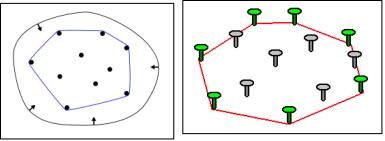
\includegraphics{ch1.jpg}
        \label{ch1}
        \caption{تعریف اولیه‌ی پوش محدب}
    \end{center}
\end{figure}

تعريف فوق، براي پوش محدب تعدادي نقطه در فضاي سه‌بعدي نيز صادق است. در حقيقت پوش محدب تعدادي نقطه در فضاي سه‌بعدي، عبارت است از پوش بدست‌آمده با کشيدن يک پوشش لاستيکي به دور نقاط در فضاي سه بعدي.

\begin{defn}
    پوش محدب مجموعه نقاط $S$ در صفحه، برابر است با اجتماع کليه مثلث‌هاي تشکيل‌شده با کمک نقاط $S$ .
\end{defn}

مشابه تعاريفي که براي پوش محدب مجموعه‌اي از نقاط گفته شد، مي‌توان پوش محدب يک چندضلعي غير محدب را نيز تعريف کرد. تعاريف زير، که همه با هم معادل هستند، نه تنها براي پوش محدب يک مجموعه از نقاط در صفحه، بلکه براي پوش محدب يک چندضلعي غير محدب نيز صحيح مي‌باشند. از طرف ديگر نه تنها در فضاي دو بعدي، بلکه براي کليه ابعاد قابل توسعه هستند. درکليه تعاريف زير،  $S$ هم مي‌تواند مجموعه‌اي از نقاط در صفحه باشد و هم يک چندضلعي غير محدب. 

\begin{defn}
    پوش محدب مجموعه‌ي  برابر است با $S$ اشتراک کليه مجموعه‌هاي محدب شامل $S$ .
\end{defn}

با کمک تعاريف بالا، بعضي از ويژگي‌هاي يک چندضلعي محدب نيز مشخص مي‌شود. اکنون سؤال اين است که اگر يک چندضلعي داده شود، چگونه مي‌توان بررسي کرد که اين چندضلعي محدب است يا خير. به عبارت ديگر، ما به معياري نياز داريم که بتوانيم محدب بودن يک چندضلعي را تشخيص دهيم. تعريف زير معياري به دست مي‌دهد که با کمک آن مي‌توان محدب‌بودن يک چندضلعي را بررسي نمود.

\begin{defn}
    چندضلعي $P$ محدب است اگر و تنها اگر براي هر دو نقطه درون $P$ پاره‌خطي که آن‌ها را به هم وصل مي‌کند، درون $P$ قرار گيرد.
    
    $$\forall x, y \in P; \bar{xy} \in P$$
\end{defn}


از اين تعريف بدست مي‌آيد که يک چندضلعي محدب داراي دندانه و زاويه انعکاسي (زاويه بيش از 180 درجه) نيست. زيرا اگر چندضلعي دندانه داشته باشد و $x$ و $y$ دو طرف دندانه باشند، آنگاه وجود دندانه و يا زاويه انعکاسي موجب مي‌شود بخشي از خط $\bar{xy}$ خارج از چندضلعي قرار گيرد.

با توجه به تعريف رؤيت‌پذيري، مي‌توان گفت چند P  محدب است؛ اگر و تنها اگر هر دو نقطه x و y درون P براي يکديگر رؤيت‌پذير باشند.

براي
$\alpha+\beta =1$ و $\alpha,\beta \ge 0$ ، $\alpha x + \beta y$
عبارت است از پاره‌خط واصل بين دو نقطه $x$ و $y$. بنابراين در تعريف بالا، شرط لازم و کافي براي محدب بودن $P$ آن است که براي هر دو نقطه
$x$ و $y$
درون $P$ پاره‌خط
$\alpha x + \beta y$
براي
$\alpha,\beta \ge 0$ و $\alpha+\beta =1$
درون چندضلعي $P$ قرار گيرد.

از سوي ديگر، با قراردادن مقادير متفاوت براي $\alpha$ و  $\beta$ مي‌توان حالت‌هاي خاصي از رابطه بالا را بدست آورد.

\begin{figure}[h!]
    \begin{center}
        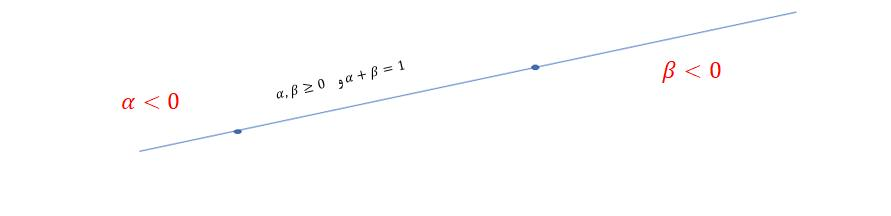
\includegraphics[width=\linewidth]{line_param.jpg}
        \label{line_param}
        \caption{نمايش بخش‌هاي مختلف يک خط با توجه به مقدار پارامتر}
    \end{center}
\end{figure}

\begin{itemize}
    \item
    اگر قرار دهيم $\alpha=0$($\beta=0$) در اين صورت $\alpha x + \beta y$ معادل نقطه $x$ ($y$) خواهد بود. 
    \item
    اگر قرار دهيم $\alpha=\beta=\frac{1}{2}$ نقطه $\frac{\alpha+\beta}{2}$ بدست مي‌آيد.
    \item
    اگر اجازه دهيم $\alpha,\beta \ge 0$ باشد، سمت چپ و سمت راست پاره‌خط بدست مي‌آيد. بطور مشابه، براي $\beta<0$ سمت چپ و براي $\alpha<0$  سمت راست پاره‌خط بدست خواهد آمد.
\end{itemize}

تعريف فوق را براي فضاهاي با ابعاد بيشتر از 2 نيز قابل تعميم مي‌باشد.

\begin{defn}
    فرض کنيد $S=\{x_1, x_2, ...,x_k\}$ آنگاه يک ترکيب محدب از مجموعه $S$ در صفحه عبارت است از:
    
    $$ \sum_{i=1}^k\alpha_i x_i \quad S.T. \quad  \sum{\alpha_i}=1 \quad and \quad \alpha_i>0$$
\end{defn}


در تعريف بالا حالت هاي خاص زير قابل توجه است: 
\begin{itemize}
    \item
    ترکيب محدب دو نقطه يک خط مي‌باشد.
    \item
    ترکيب محدب سه نقطه يک مثلث مي‌شود.
    \item
    ترکيب محدب چهار نقطه در صفحه، يک چهارضلعي محدب و در فضاي سه بعدي  يک چهار وجهي محدب مي‌باشد که يک 3-سيمپلکس ناميده مي‌شود.
    \item
    ترکيب محدب $d+1$ نقطه، در فضاي $d$ بعدي شکل مي‌گيرد که يک d-simplex ناميده مي‌شود.
\end{itemize}

در بخش بالا، تعاريف متعددي براي پوش محدب و چندضلعي محدب ارائه شد. بعضي از اين تعاريف با هم شباهت دارند و بعضي کاملا متفاوت اند. پرسشي که ممکن است مطرح باشد، اين است که کدام يک از اين تعاريف بهتر و مناسب‌تر است. پرسش ديگري که به دنبال اين پرسش مي تواند مطرح شود، اين است که در اينجا معيار بهتر و مناسب‌تر بودن براي يک تعريف چيست؟ آيا تعريفي که قابل‌ فهم‌تر و ساده‌تر باشد مناسب‌تر است يا تعريفي که بتوان آن را به صورت يک فرمول نوشت و يا تعريفي که به جاي توصيف به صورت رياضي قابل بيان باشد؟ بدون شک زيبايي، سادگي و مناسب‌تر بودن، در گرايش‌هاي علمي متفاوت يکسان نيست. به عنوان مثال، تعاريف 3 و 4 از نظر رياضي بسيار ساده و قابل فهم اند و از نظر يک رياضيدان به سادگي قابل توصيف مي‌باشند. در حالي که از نظر يک متخصص کامپيوتر و متخصص تکنولوژي اطلاعات، هيچ کدام تعاريف مناسبي نيستند؛ زيرا تعداد مجموعه‌هاي محدب $P$ که شامل $S$ باشند مي تواند بي‌شمار باشد؛ در اين حالت، چگونه مي‌توان يک برنامه کامپيوتري نوشت و يا يک آلگوريتم محاسباتي ارائه داد که بتواند از ميان چندضلعي‌هاي محدب شامل $S$ چندضلعي که کمترين مساحت و يا محيط را دارد پيدا کند؟

در حالي که تعريف شماره 2 که در يک نگاه از نظر رياضي ساده به نظر نمي‌رسد، مي تواند به طراحي يک روش محاسباتي  براي يافتن پوش محدب مجموعه‌اي از نقاط بيانجامد. در واقع مي‌توان کليه مثلث‌هاي تشکيل‌شده با کمک نقاط $S$ را بدست آورد، سپس از آن‌ها اجتماع گرفت. تعداد اين مثلث‌ها برابر کليه ترکيبات 3 تايي خواهد بود و در زمان $O(n^3)$ قابل محاسبه است. بنابراين، تعريف شماره 2 از نظر محاسباتي مناسب‌تر است و بر اساس آن مي‌توان الگوريتمي براي محاسبه پوش محدب بدست آورد

پرسش فوق مي تواند در تمام بخش‌هاي اين کتاب مطرح شود. در بعضي تعاريف و قضايا ممکن است استدلال ساده‌تر و يا زيباتري وجود داشته باشد و قابل فهم‌تر هم باشد، اما در اين کتاب تعريف و يا پاسخي بهتر و مناسب تر است که توسط يک آلگوريتم قابل بيان و توسط ماشين قابل پياده شدن باشد. 

در حالتي که $S$ مجموعه‌اي از نقاط در فضاي با ابعاد بالاتر باشد، تعريف زير را مي توان تعميم تعريف شماره 2 دانست.

\begin{defn}
    فرض کنيد $S$ مجموعه‌اي از نقاط در فضاي d-بعدي باشد. در اين صورت، پوش محدب مجموعه $S$، برابر است با مجموعه کليه ترکيبات محدب  $d+1$ (يا کمتر) نقطه از $S$. در حالت خاص، پوش محدب $S$ برابر است با کليه –dسيمپلکس‌هاي توليدشده با کمک نقاط $S$.
\end{defn}


اکنون سعي مي کنيم راهي براي ساختن رويه محدب مجموعه از نقاط که در صفحه داده شده است بيابيم. براي اين منظور به تعريف نقطه مرزي مي‌پردازيم و با کمک آن، اولين و ساده‌ترين روش ساختن پوش محدب را بيان مي‌کنيم.

\begin{defn}
    نقطه مرزي \footnote{Extreme Points}:
    نقطه $s \in S$ يک نقطه مرزي براي مجموعه $S$ است، اگر خط جهت دار $\Gamma$ وجود داشته باشدکه از نقطه $s$ عبور کند و تمام نقاط مجموعه $S$ روي يا سمت چپ  باشند.
\end{defn}

به سادگي مي‌توان نشان داد تمام نقاط روي مرز يک پوش محدب، نقاط مرزي هستند. (تمرين)

در تعريف بالا مي توانستيم خط $\Gamma$ را جهت دار در نظر نگيريم و در عوض ديگر نمي توانستيم بگوييم تمام نقاط مجموعه $S$ روي يا سمت چپ $\Gamma$ باشند. بلکه بايد مي گفتيم تمام نقاط مجموعه $S$ يک سمت  قرار گيرند.

براي يافتن پوش محدب يک مجموعه از نقاط، کافي است نقاط مرزي آن را داشته باشيم. زيرا در اينصورت با اتصال نقاط مرزي به يکديگر، مي‌توان پوش محدب را بدست آورد. اين مسئله در مورد يک مجموعه غير محدب نيز صادق است؛ به عبارت ديگر با اين روش يعني اتصال کليه نقاط مرزي مي‌توان پوش محدب يک مجموعه نامحدب را نيز بدست آورد.

دسترسي به بعضي از نقاط مرزي، چندان دشوار نيست؛ به عنوان مثال، نقطه‌اي که بيشترين مولفه (هم‌چنين کمترين مولفه) $y$ را دارد، يک نقطه مرزي است. اگر چه چنين نقطه‌اي ممکن است منحصر به فرد نباشد، با اين حال طبق تعريف باز هم نقطه مرزي محسوب مي‌شود. همچنين چپ‌ترين و راست‌ترين نقاط S نيز جزء نقاط مرزي هستند. مشابه حالت قبلي، اگر چنين نقطه‌اي منحصر به فرد نباشد، باز هم نقطه مرزي محسوب مي‌شود. زيرا در هر کدام از حالات مي توان خطي را رسم کرد که کليه نقاط در يک سمت آن باشند.

با اتصال اين چهار نقطه يعني چپ ترين، راست ترين، بالاترين و پائين ترين نقطه يک چهارضلعي محدب بدست مي‌آيد که اگر چه يک تقريب نه چندان مناسب براي پوش محدب است لاکن نقطه شروع يافتن پوش محدب به روش "پوش سريع" مي‌شود

\colorbox{yellow}{که در بخش هاي بعدي توضيح مي‌دهيم.}

اکنون با استفاده از تعريف نقطه مرزي بدنبال روشي هستيم که بتواند بين نقاط مرزي و غير مرزي تمايز ايجاد کنيم. چرا که در حقيقت اين نقاط مرزي هستند که پوش محدب را مي سازند. تعريف ارائه شده در بالا براي نقطه مرزي مستقيما نمي تواند يک روش محاسباتي به‌دست دهد. زيرا يافتن يک خط در يک نقطه که کليه نقاط روي يا در يک سمت آن قرار گيرد را نمي توان به سادگي به شکل محاسباتي نوشت. اما برعکس ممکن است از اين نکته بتوان استفاده کرد که نقطه‌اي که درون يک چندضلعي براي مثال يک مثلث باشد نمي تواند يک نقطه مرزي باشد زيرا هر خطي که از آن نقطه عبور مي‌کند بخشي از رؤس را در يک سمت و بخش ديگر را در سمت ديگر خواهد داشت. اين نکته کمک مي کند که بتوانيم  لم زير را بيان کنيم.

هر سه نقطه عضو مجموعه $P$ تشکيل يک مثلث مي‌دهند؛ بنابراين اگر تمام نقاط سه‌گانه را بررسي کنيم و نقطه $x$ متعلق به هيچ کدام نباشد، با توجه به لم فوق مي‌توان گفت که $x$ يک نقطه مرزي است.

\begin{figure}[h!]
    \begin{center}
        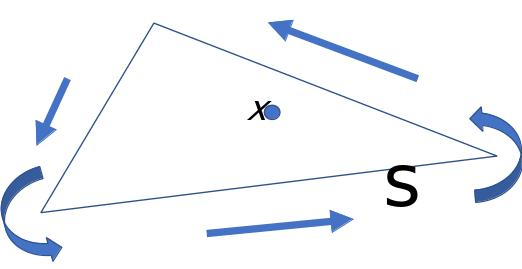
\includegraphics[width=\linewidth]{left_line.jpg}
        \label{left_line}
        \caption{چنانچه نقطه $x\in P$  باشد، آنگاه x سمت چپ کليه اضلاع مثلث خواهد بود}
    \end{center}
\end{figure}

اگر جهت چپ‌گرد را بر روي اضلاع مثلث در نظر بگيريد، چرخش روي اضلاع در جهت خلاف حرکت عقربه‌هاي ساعت خواهد بود. چنانچه $x\in P$ باشد، آنگاه $x$ سمت چپ کليه اضلاع مثلث خواهد بود. اين مي‌تواند يک معيار به دست دهد که با کمک آن مرزي‌بودن و يا مرزي‌نبودن يک نقطه را بررسي نماييم. به عبارت ديگر خواهيم داشت:  $x\in P$ اگر و تنها اگر $x$ سمت چپ اضلاع مثلث باشد. بنابراين مي‌توان الگوريتم زير را نوشت.

\begin{latin}
\begin{verbatim}
Algorithm Extreme Point:

for each i do
    for each  j ≠ i do
      for each k ≠ j ≠ i do
        for each l ≠ k ≠ j ≠ i do
          if Pi is left or on ( P_j P_k ) and
             Pi is left or on ( P_k P_l ) and
             Pi is left or on ( P_l P_j )
                                  then Pl is none extreme
\end{verbatim}
\end{latin}

با توجه به آلگوريتم فوق، بررسي مرزي ‌بودن براي يک نقطه در زمان $O(n^3)$ صورت مي‌گيرد. زيرا بايد تمام مثلث هاي موجود که تعداد آنها ترکيب 3 از $n$ است را بررسي کنيم. در‌نتيجه اگر کليه نقاط مرزي را بدست مي‌آوريم. براي اين امر، زمان$ O(n^4)$ لازم است و از آنجا که با بدست‌آوردن کليه نقاط مرزي مي‌توان پوش محدب مجموعه‌اي از نقاط را بدست آورد، با اين روش، پوش محدب در زمان $O(n^4)$ بدست مي‌آيد.

آنچه گفته شد، يک روش براي محاسبه نقاط مرزي و به دنبال آن پوش محدب نقاط خواهد بود؛ اگر چه اين زمان ابدا زمان مناسبي نيست و در آينده، پوش محدب را در زمان خيلي بهتري محاسبه خواهيم کرد.

اکنون با الهام از تعريف نقطه مرزي، ضلع مرزي را تعريف مي‌کنيم.

تعريف ضلع مرزي واضح‌تر از نقطه مرزي است و کمک مي کند پوش محدب را در زمان بهتري بدست آوريم. 

\begin{defn}
    تعريف ضلع مرزي \footnote{Extreme Edges}:
    ضلع مرزي مجموعه $S$ ، پاره خطي است مانند $\Delta$ كه تمام نقاط $S$ روي يا يك طرف خطي باش که از $\Delta$  عبورمي کند. 
\end{defn}

\begin{latin}
\begin{verbatim}
Algorithm Extreme edges:

  for i and j ≠ i 
      for each k ≠ j ≠ i do
         if Pk is not left or on ( P_i P_j )
                                   then ( P_i P_j ) is none extreme 
\end{verbatim}
\end{latin}

با توجه به آلگوريتم فوق، ديده مي‌شود که بررسي مرزي‌بودن يک خط در زمان $O(n)$ صورت مي‌پذيرد. با توجه به اينکه هر زوج نقطه‌ مي‌تواند کانديداي خط مرزي باشد، بنابراين $O(n^2)$ کانديداي خط مرزي وجود دارد. لذا زمان لازم براي بدست آوردن کليه اضلاع مرزي، $O(n^3)$ خواهد بود. از آنجا که اضلاع مرزي پوش محدب را مي‌سازند، با کمک آلگوريتم فوق مي‌توان پوش محدب مجموعه‌اي از نقاط را بدست آورد. بنابراين پوش محدب در زمان  $O(n^3)$ بدست مي‌آيد. اگر چه بدست‌آوردن پوش مرزي با اين روش، از زمان $O(n^4)$ بهتر است، ولي باز هم زمان مناسبي براي محاسبه پوش محدب نيست.

اکنون با تعاريف فوق وقت آن رسيده است که اولين آلگوريتم کارا براي محاسبه پوش محدب مجموعه‌اي از نقاط را ارائه نماييم. پيچيدگي زمان اين الگوريتم که نوعي الگوريتم افزايشي است، بهينه خواهد بود.

چنانچه توضيح داده شد آلگوريتم بدست‌آوردن پوش محدب به روش افزايشي، روش ساده‌اي است که از اصول اوليه روش افزايشي استفاده مي‌کند. در اين روش، نقاط را يکي‌يکي اضافه مي‌کنيم و پوش محدب مجموعه جديد را به روز مي‌نماييم. اين عمل را تا وقتي تکرار مي‌کنيم که ديگر نقطه‌اي باقي نماند. اين روش براي نقاط در فضاي سه بعدي ($R^3$) نيز قابل تعميم است. کليات آلگوريتم به شکل زير است:

الگوريتم افزايشي يافتن پوش محدب:

\begin{itemize}
    \item
    ابتدا با يک نقطه شروع مي‌کنيم. سپس نقطه دوم و پس از آن، نقطه سوم را اضافه مي‌نماييم.
    \item
    پوش محدب سه نقطه را - که يک مثلث است - بدست مي‌آوريم.
    \item
    نقاط را يکي‌يکي اضافه مي‌کنيم، پوش محدب قبلي را به روز مي‌کنيم و پوش محدب جديد را بدست مي‌آوريم.
    \item
    فرض کنيد تا کنون $i$  نقطه بررسي و پوش محدب در مرحله $i$  ام ساخته شده است؛ با اضافه‌کردن نقطه $i+1$ ام يعني نقطه $p_i$ بررسي‌هاي لازم در مورد اين نقطه صورت مي‌گيرد. دو حالت ممکن است اتفاق بيفتد:
    \begin{itemize}
        \item
        چنانچه $p_i$ داخل پوش بدست‌آمده تا مرحله قبلي باشد، پوش محدب تغييري نخواهد کرد و پوش محدب جديد، همان پوش محدب قبلي خواهد بود.
        \item
        چنانچه $p_i$ داخل پوش بدست‌آمده تا مرحله قبلي نباشد، براي توسعه پوش محدب و افزودن نقطه    $i+1$  ام، بايد از نقطه $p_i$ مماس‌هايي بر پوش محدب قبلي رسم و چندضلعي را تکميل کنيم
    \end{itemize}
\end{itemize}

فرض کنيد $i$ نقطه تا کنون بررسي شده است و پوش محدب اين نقاط محاسبه گرديده است. براي تکميل مرحله $i+1$ ام، دو سؤال مطرح است که بايد به آن‌ها پاسخ دهيم.

سؤال اول اين است که چگونه و در چه زماني مي‌توان تشخيص دهيم كه نقطه $p_i$ داخل پوش محدب $i$ نقطه قبلي قرار دارد؟

سؤال دوم اين است که از نقطه $p_i$  خارج پوش محدب بدست‌آمده توسط $i$ نقطه قبلي چگونه و در چه زماني مي‌توان مماس‌هايي بر پوش محدب رسم كرد؟

اين دو سؤال را به صورت دو مسئله مستقل مطرح و حل مي‌کنيم.

\subsection{موقعيت يک نقطه نسبت به چندضلعي محدب}

چند ضلعي محدب $P$  و نقطه$ p_i$ داده شده است. بررسي نماييد که آيا $p_i\in P$  است؟

حل: يک جهت بر روي اضلاع چندضلعي در نظر مي‌گيريم. اين جهت معمولا چپ‌گرد و بر خلاف حرکت عقربه‌هاي ساعت است. به وضوح روشن است که$p_i\in P$  برقرار خواهد بود. اگر $p_i$ سمت چپ و يا روي کليه اضلاع $P$ باشد، اين مي‌تواند يک معيار به دست دهد که با کمک آن، درون و يا بيرون بودن يک نقطه نسبت به يک چندضلعي محدب بررسي شود.

بنابراين تشخيص اينکه آيا نقطه pi درون يک چندضلعي محدب با $n$ ضلع واقع شده است يا خير، در زمان $O(n)$  انجام مي‌شود.

\begin{latin}
\begin{verbatim}
Algorithm left of edges:

for each edge e of boundary of polygon P do
        if P_i is left or on e 
                                    then p_i is in P
\end{verbatim}
\end{latin}

\subsection{رسم مماس بر يک چندضلعي}

چند ضلعي $P$ و نقطه $p \notin P$ خارج چندضلعي داده شده است. در اين حالت مي‌توان دو مماس از $p$  به $P$  رسم نمود. الگوريتمي براي رسم اين دو مماس ارائه دهيد.
حل: بدون شک يک مماس از نقطه $p$  بر چندضلعي $P$، از يکي از رئوس $P$ خواهد گذشت. در حالتي خيلي خاص، ممکن است مماس از يک ضلع عبور کند که آن را ناديده مي‌گيريم؛ چرا که در اين حالت بايد سه نقطه از مجموعه نقاط، روي يک خط واقع شده باشند و بنا به فرض، اين حالت مستثني شده است.

مسئله به دو روش قابل حل است که هر دو را مي‌توان پياده‌سازي و اجرا نمود.

روش اول: واضح است که هر خط که از نقطه $p$  به يکي از رئوس چندضلعي $P$ متصل شود،  رئوس $P$ را به دو بخش تقسيم مي‌کند. بخشي از نقاط در يک سمت (سمت راست)  و بخشي ديگر در سمت ديگر نقاط (سمت چپ) خط واصل خواهند بود. مشخصا چنانچه خطي که از $p$ به چندضلعي وصل و مماس نباشد و از رأس $p_i$  عبور کند، آنگاه $p_{i-1}$ يک سمت خط $pp_i$ خواهد بود و $p_{i+1}$ سمت ديگر آن. در حاليکه اگر $pp_i$ يک خط مماس بر چند ضلعي P باشد، آنگاه شرايط به گونه ديگري است. در واقع چنانچه خط $pp_i$ از $p$ به چندضلعي متصل و در رأس$p_i$  بر آن مماس باشد. در اين صورت $p_{i-1}$ و $p_{i+1}$ هر دو يک سمت $pp_i$ خواهند بود. اين يک معيار مناسب است که با اتصال خطوط از نقطه $p$ به رأس $p_i$ و بررسي وضعيت نقاط قبل و بعد از $pi$ نسبت به خط $pp_i$ مي تواند به تشخيص مماس کمک کند.

\begin{figure}[h!]
    \begin{center}
        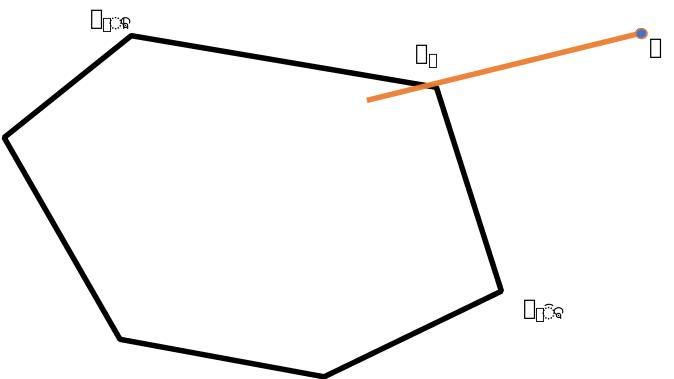
\includegraphics[width=\linewidth]{momas_2.jpg}
        \label{momas_2}
        \caption{رئوس در يک سمت قرار دارند.}
    \end{center}
\end{figure}

\begin{figure}[h!]
    \begin{center}
        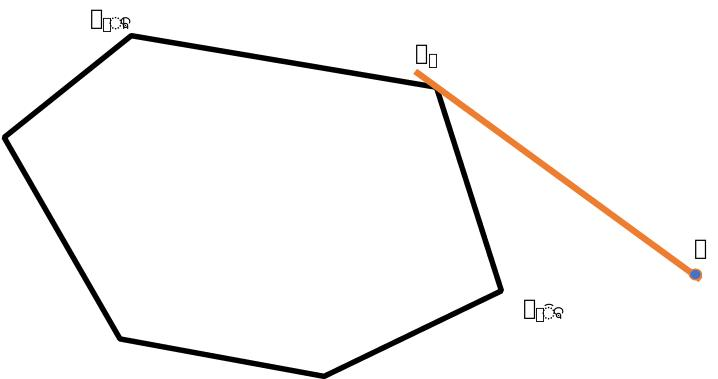
\includegraphics[width=\linewidth]{momas_1.jpg}
        \label{momas_2}
        \caption{رئوس در دو سمت خط هستند.}
    \end{center}
\end{figure}

روش دوم: فرض کنيد خطي از نقطه $p$ به يکي از رئوس چندضلعي $P$ مانند رأس$p_i$  رسم و از آن عبور کند و بر چندضلعي مماس نباشد. در اين صورت نقطه $p$ سمت راست هر دو ‌خطي خواهد بود که از امتداد اضلاع $p_{i-1}p_i$ و $p_ip_{i+1}$ بدست آمده اند. در حالي‌ که اگر خطي که از نقطه p  به يکي از رئوس چندضلعي P مانندpi  متصل شود و بر آن مماس باشد، در اين حالت نقطه p سمت راست خطي خواهد بود که از $p_{i-1}p_i$ مي گذرد و سمت چپ خطي که از $p_ip_{i+1}$ مي گذرد.

بنابراين با کمک دو روشي که ارائه شد مي توان خط مماس بر چندضلعي را از خطي که به يک رأس متصل شده و چندضلعي را قطع کرده است از خط مماس متمايز نمود.

از آنجا که براي يافتن يک مماس با کمک هر کدام از دو روش بايد يکي يکي براي تمامي رؤس‌ $p_i$ وضعيت خط $pp_i$ را نسبت به رؤس و يا اضلاع قبل و بعد از $p_i$ بررسي نمود بنابراين اينکار در زمان $O(n)$   انجام مي شود. 

چنانچه مماس‌ها از نقطه $p$ بر چندضلعي $P:p_0,p_1,…, p_{i-1}, p_i, p_{i+1}, p_{j-1}, p_j, p_{j+1},…,p_k$ به ترتيب از رئوس $p_i$ و  $p_j$گذشته باشد، در اين صورت  $p$ با کمک مماس‌ها يک چندضلعي جديد خواهد ساخت که جاي چندضلعي  قبلي را مي گيرد و رئوس آن به صورت $(p_0,p_1,…, p_{i-1},p_i,p,p_j, p_{j+1},…,p_k)$ خواهند بود.    

$(p_0,p_1,…, p_{i-1}, p_i, p_{i+1}, p_{j-1}, p_j, p_{j+1},…,p_k) \rightarrow (p_0,p_1,…, p_{i-1},p_i,p,p_j, p_{j+1},…,p_k)$

\subsection{الگوريتم پوش محدب افزايشي}

با کمک نقاط  $p_2,  p_1, p_0$, $H_2 = CH(p_0, p_1, p_2)$ ، پوش محدب اين سه نقطه را  که يک مثلث است مي‌سازيم.

در مرحله$i+1$  ام، به فرض $Q=H_i-1$ پوش محدب $i$  نقطه باشد.
با اضافه‌شدن نقطه $i+1$ ام $P=P_i$ مي‌خواهيم $H=CH(Q\cup\{p\})$ را بدست ‌آوريم.
يکي از دو حالت زير ممکن است رخ دهد:

حالت اول: اگر $p \in Q$ ، در اين صورت $H=H_k-1$

حالت دوم: اگر $p \notin Q$ ، در اين حالت دو مماس از $p$ به دو نقطه مرزي وصل مي‌کنيم.

براي رسم مماس از $p$ به $Q$ ، فرض کنيد $p_i$ يکي از رئوس $Q$ محل تماس مماس باشد. در اين صورت $p$ بايد سمت چپ (راست) $p_{i-1}p_i$ و سمت راست (چپ) $p_ip_{i+1}$ باشد. در نتيجه اگر $p_i$ و $p_j$ دو نقطه تماس مماس‌ها از نقطه $p$ باشند، آنگاه:

$(p_0,p_1,…, p_{i-1}, p_i, p_{i+1}, p_{j-1}, p_j, p_{j+1},…,p_k) \rightarrow (p_0,p_1,…, p_{i-1},p_i,p,p_j, p_{j+1},…,p_k)$

\begin{latin}
\begin{verbatim}
Algorithm: Tangent Points:

for  i = 0 to n-1 do
    if  XOR ( p left or on  ( p_i-1 , p_i ) , p left or on   ( p_i , p_i+1 )  )  
        then p_i  is point of Tangent
\end{verbatim}
\end{latin}

\subsection{پيچيدگي زمان آلگوريتم}

زمان لازم براي بررسي اينکه نقطه $p_i$ داخل پوش محدب $i$ نقطه قبلي قرار دارد يا خير:  $O(i)$ 

زمان لازم براي رسم مماس‌هاي $p_i$ بر پوش محدب $i-1$ نقطه قبلي: $O(i)$ 

بنابراين زمان کلي آلگوريتم عبارت خواهد بود از $T(n^2)=3+4+…+n=O(n^2)$

مي‌توان با کاهش زمان ترسيم مماس، زمان آلگوريتم را به $O(nlogn)$ کاهش داد.

\begin{figure}[h!]
    \begin{center}
        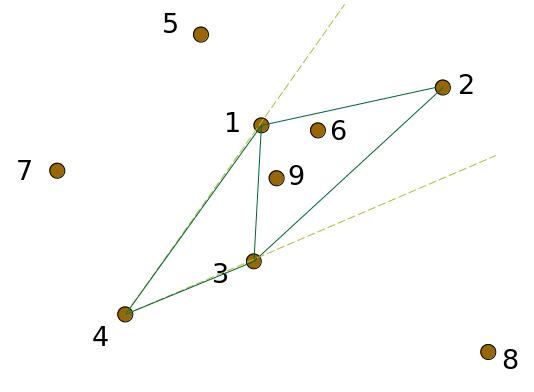
\includegraphics[width=\linewidth]{ch2.jpg}
        \label{ch2}
        \caption{مراحل افزايش پوش محدب}
    \end{center}
\end{figure}

مسئله 3: نشان دهيد هر چندضلعي محدب پروانه‌اي شكل است.

مسئله 4: نشان دهيد هر چندضلعي پروانه‌اي، ستاره‌شكل است؛ در حالي که هر چندضلعي ستاره‌اي شکل، لزوما پروانه‌اي شکل نمي‌باشد. 

مسئله1 : چندضلعي محدب $P$ و نقطه $p$ خارج چندضلعي ($p\notin P$) داده شده است. نشان دهيد تنها مي‌توان دو مماس از $p$  به $P$ رسم نمود. 

مسئله2 : چندضلعي غير محدب $P$ و نقطه $p$ خارج چندضلعي ($p\notin P$) داده شده است. چه تعداد مماس از $p$  مي‌توان به $P$ رسم نمود؟ (در دو حالت مي‌توان به اين پرسش پاسخ داد. يک حالت، مماس‌هايي که $P$ بطور کامل يک سمت آن‌ها واقع شود و حالت ديگر اينکه لزوما$P$  يک سمت مماس قرار نگيرد.)

مسئله3 : با استفاده از تعريف نشان دهيد تمام نقاط روي مرز يک چندضلعي محدب، نقاط مرزي هستند. 

مسئله4 : مجموعه نقاط $S$ داده شده است. نقطه $x\in S$ در اين مجموعه يک نقطه مرزي نيست؛ اگر و فقط اگر داخل يک مثلث (بسته) باشد كه رئوسش از نقاط $S$ هستند و $x$ خود يكي از رئوس مثلث نيست. 

مسئله5 : مجموعه نقاط $S$ داده شده است. با مرتب‌کردن نقاط مجموعه $S$ ديگر نيازي نيست در هر مرحله بررسي نماييم که آيا نقطه $p_i$ داخل پوش محدب $i$ نقطه قبلي قرار دارد يا خير و با اين کار، زمان آلگوريتم ممکن است کاهش يابد. آلگوريتمي بنويسيد که اين کار را انجام دهد. 

مسئله6 : نشان دهيد تعريف زير براي پوش محدب مجموعه نقاط $S$ صحيح است:
 "پوش محدب مجموعه نقاط $S$ در صفحه، برابر است با بزرگترين مجموعه محدب که رئوسش همگي از نقاط $S$ باشد."

مسئله7 : نشان دهيد تعريف زير براي پوش محدب مجموعه نقاط $S$ صحيح است:

"پوش محدب مجموعه‌اي از نقاط يا مجموعه غير محدب $S$ برابر است با مجموعه محدب P شامل $S$ با کمترين مساحت يا محيط."

\section{موقعيت يك نقطه نسبت به يک چندضلعي}

مسئله سوم هندسي که با روش افزايشي حل مي کنيم مسئله موقعيت يك نقطه نسبت به يک چندضلعي مي باشد. صورت کلي مسئله به صورت زير است.
چندضلعي $P$ که مي تواند غير محدب باشد و نقطه $q$ در صفحه داده شده است. سؤال اين است که آيا نقطه $q$ درون چندضلعي است يا خارج آن ؟

\subsection{مقدمه و کاربرد}

تعيين موقعيت يک نقطه در صفحه از مباحث مهم و جذاب هندسه است با کاربردهاي بسيار در جغرافيا، علوم طبيعي و نظامي. که بدليل اينکه از موضوع اين مبحث خارج است نمي توانيم فعلا به آن بپردازيم. اگر چه اين موضوع مهم و ارزشمند است، لاکن تعيين موقعيت يک نقطه در يک نقشه پيچيده هندسي مي‌تواند مهم و در عين حال نزديک به موضوع اين بخش باشد. براي ساده‌کردن مسئله مي‌توان يک نقشه پيچيده هندسي را با يک چندضلعي ساده تقريب کرد. اگر چندضلعي محدب باشد، مشخص‌کردن اينکه يک نقطه در داخل چندضلعي است و يا در خارج آن، کار چندان دشواري نيست. ولي اگر چندضلعي غير محدب و بسيار پيچيده باشد، مسئله مي‌تواند جدي‌تر به نظر آيد. به عنوان مثال، به شکل 11 توجه کنيد. با يک نگاه ساده نمي‌توان مشخص نمود که نقطه خارج چندضلعي است و يا داخل آن. 

\begin{figure}[h!]
    \begin{center}
        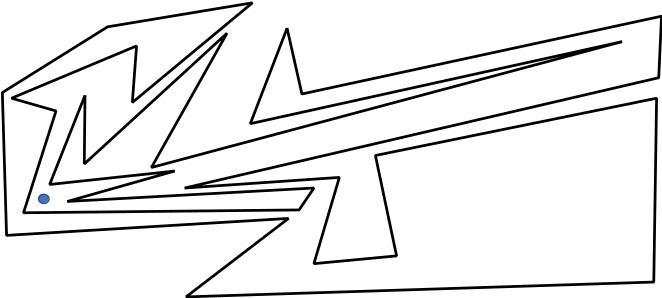
\includegraphics[width=\linewidth]{pimp.jpg}
        \label{pimp}
        \caption{به سادگي نمي‌توان نسبت به موقعيت نقطه نسبت به چند ضلعي نظر داد.}
    \end{center}
\end{figure}

اگر $P$ محدب باشد، براي پاسخ به اين سؤال مي‌توان با استفاده از روش بررسي چپ بودن يعني بررسي اينکه نقطه $q$ سمت چپ کليه اضلاع چندضلعي هست يا خير در مورد موقعيت نقطه نسبت به چندضلعي نظر داد. بررسي موقعيت نقطه $q$ نسبت به هر ضلع، در زمان ثابت انجام مي‌شود. بنابراين اگر $P$ محدب باشد، به زمان $O(n)$ براي بررسي موقعيت يک نقطه نسبت به يک چندضلعي نياز داريم. اگر چه با کمک يک روش ابتکاري و جذاب، مي‌توان زمان را تا $O(logn)$ بهبود بخشيد.

روش فوق، در حالت کلي براي چندضلعي غيرمحدب مفيد نخواهد بود. به عنوان مثال، در چندضلعي غيرمحدب نقطه a سمت راست ضلع $e$ قرار دارد؛ در حالي که داخل چندضلعي مي‌باشد و اساسا بخشي از چندضلعي، سمت چپ پاره‌خط $e$ و بخشي سمت راست آن قرار دارد. بنابراين "روش بررسي چپ بودن" روش مناسبي براي بررسي موقعيت يک نقطه نسبت به يک چندضلعي غير محدب نيست.

\begin{figure}[h!]
    \begin{center}
        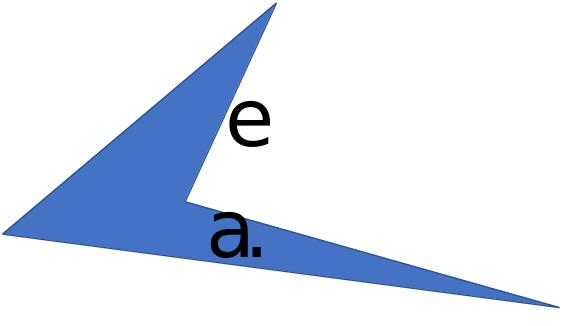
\includegraphics[width=\linewidth]{not_hull.jpg}
        \label{not_hull}
        \caption{بخشي از چندضلعي، سمت چپ پاره‌خط $e$ و بخشي سمت راست آن قرار دارد.}
    \end{center}
\end{figure}

در حالت کلي دو روش متفاوت براي حل مسئله  فوق وجود دارد. روش "ارسال پرتو" \footnote{Ray shooting method}
و "روش زاويه" \footnote{Signed angle method}
. ما در اين بخش به توضيح روش ارسال پرتو مي پردازيم و بخش بعدي را به روش زاويه اختصاص خواهيم داد

\subsection{آلگوريتم ارسال پرتو براي تعيين موقعيت يك نقطه نسبت به چندضلعي}

\begin{figure}[h!]
    \begin{center}
        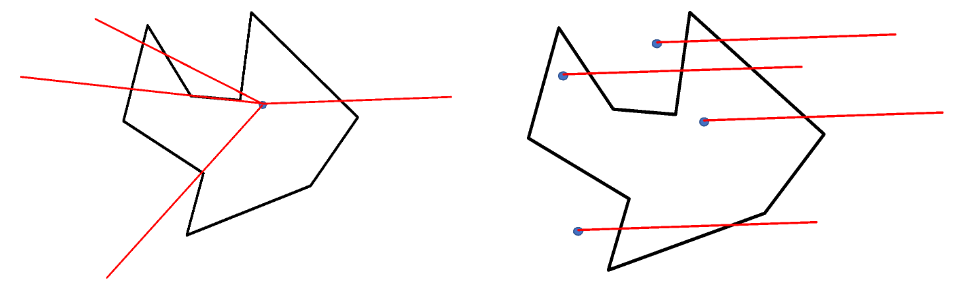
\includegraphics[width=\linewidth]{ray.png}
        \label{ray}
        \caption{يک شعاع پرتو از نقطه  $q$ که تا بينهايت امتداد دارد رسم مي‌کنيم. با توجه به تعداد تقاطع‌هاي اين شعاع پرتو با مرز چندضلعي، در مورد داخل و يا خارج بودن نقطه $q$ تصميم مي‌گيريم.}
    \end{center}
\end{figure}

براي اينکه آلگوريتم به درستي جواب دهد فرض کنيد $q$  خود يکي از رؤس نيست و نيز $q$ همراستا با يکي از رؤس چندضلعي نيست. نيم‌خط افقي $R$ را از $q$ در جهت مثبت محور x-ها رسم مي‌کنيم. در حقيقت اين يک شعاع پرتو خواهد بود که تا بينهايت امتداد خواهد داشت و مرز چندضلعي را قطع خواهد کرد. يک ضلع از چندضلعي، بسته به وضعيت در برخورد با شعاع پرتو، يکي از چهار وضعيت زير را خواهد داشت:

\begin{figure}[h!]
    \begin{center}
        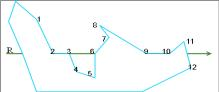
\includegraphics{intersection.jpg}
        \label{intersection}
        \caption{خط $R$ تنها با يال هاي $(1,2)$، $6,7$،$ (8,9)$ و $11,12و$ $(10,11)$ برخورد دارد}
    \end{center}
\end{figure}

\begin{itemize} 
    \item
    شعاع R ضلع را در نقطه‌اي در ميانه ضلع قطع مي‌کند. (ضلع 11-12 شکل \ref{intersection})
    \item
    شعاع R در نقطه‌اي در انتهاي (يا ابتداي) ضلع آن را قطع مي‌کند؛ يعني از يک راس عبور نمايد. (ضلع 7-6 شکل \ref{intersection})
    \item
    شعاع R از يکي از اضلاع عبور مي‌نمايد؛ يعني بر يکي از اضلاع منطبق مي‌گردد. (ضلع 9-10 شکل \ref{intersection})
    \item
    شعاع R ضلع را قطع نمي‌کند و هيچ رابطه‌اي با ضلع ندارد. (ضلع 4-5 شکل \ref{intersection})
\end{itemize}

در برخورد شعاع $R$ با مرز $\partial P$ مطابق تعريف بالا با توجه به موقعيت اضلاع و محل برخورد خط شعاع، ممکن است حالت‌هاي استثنائي پيش آيد؛ اين حالت‌ها در شکل زير نشان داده شده و تعداد برخوردها شمارش شده در زير هر يک نوشته شده است.

\begin{itemize} 
    \item
    در حالتي که تعداد برخوردها فرد باشد، $a$ داخل $P$ خواهد بود.
    \item
    در حالتي که تعداد برخوردها زوج باشد، $a$ خارج $P$ خواهد بود.
\end{itemize}


\begin{latin}
\begin{verbatim}
The ray-cutting algorithm: 

#intersection: 
        odd = inside, 
        even = outside
\end{verbatim}
\end{latin}

از آنجا که عدم دقت در شمارش تعداد برخوردهاي شعاع پرتو با پاره خط‌هاي مرز چندضلعي موجب عدم تعيين دقيق موقعيت نقطه نسبت به چندضلعي خواهد شد، بنابراين بايستي مفهوم برخورد دو پاره خط به درستي تعريف شود.

برخورد ضلع e با خط شعاع R را به شکل زير تعريف مي کنيم:

\begin{defn}
    برخورد دو خط: گوئيم ضلع e با نيم خط R برخورد دارد؛ چنانچه يک سر انتهاي e بالاي R و سر ديگرش روي يا پايين R باشد.  در شکل \ref{intersection} ، R با (1,2)، (6,7)، 11,12 و  (10,11) برخورد دارد؛ ولي با  9,10 ، 2,3 ، (3,4) و (5,6) برخورد ندارد. 
\end{defn}

در برخورد شعاع $R$ با مرز $\partial P$ مطابق تعريف بالا با توجه به موقعيت اضلاع و محل برخورد خط شعاع، ممکن است حالت‌هاي استثنائي پيش آيد؛ اين حالت‌ها در شکل زير نشان داده شده و تعداد برخوردها شمارش شده در زير هر يک نوشته شده است.

\begin{figure}[h!]
    \begin{center}
        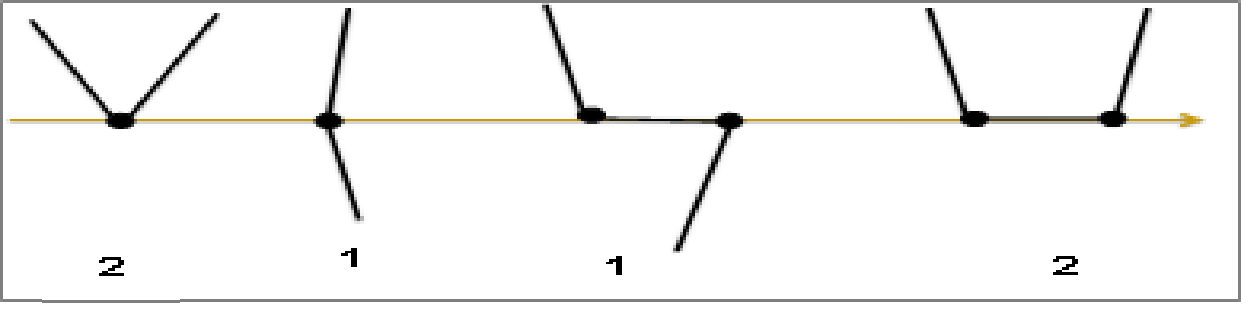
\includegraphics{inter2.jpg}
        \label{inter2}
        \caption{حالت هاي استثنايي برخورد يک خط با اضلاع چندضلعي}
    \end{center}
\end{figure}

\subsubsection{آناليز الگوريتم ارسال پرتو}

از آنجايي که مي‌توان اشتراک دو پاره‌خط را در زمان ثابت محاسبه کرد و از طرف ديگر، برخورد شعاع پرتو با کليه اضلاع چندضلعي بايد بررسي گردد، پيچيدگي الگوريتم برابر خواهد بود با:
$$T(n)=O(n)\times O(1)=O(n)$$
ممکن است اين سؤال مطرح شود که دليل اينکه اين آلگوريتم را يک روش افزايشي مي دانيم چيست. در حقيقت، آلگوريتم تقاطع شعاع پرتو با کليه اضلاع را يکي يکي بررسي مي کند تا زماني که تمام اضلاع چند‌ضلعي پيمايش شوند و آلگوريتم به انتها برسد. و تا وقتي که کليه اضلاع بررسي نشده اند هيچ پيش‌بيني صحيح نخواهد بود.

\begin{defn}
    تعريف زاويه چپ گرد: نقاط $a$، $b$ و $c$ و زاويه $\theta=\hat{acab}$  را در نظر بگيريد. زاويه  مي تواند با توجه به جهت چرخش $\hat \theta$ و علامت آن راست‌گرد يا چپ‌گرد باشد. اگر چرخش $\vec{ac}$ به سمت $\vec{ab}$ حول راس a در جهت زاويه کوچکتر پادساعتگرد باشد گفته مي‌شود زاويه منفي و اصطلاحا چپ‌گرد است. همچنين اگر چرخش ساعت‌گرد باشد، گفته مي‌شود زاويه مثبت و يا اصطلاحا راست‌گرد است.
\end{defn}

تعريف راست‌گرد يا چپ‌گرد را به صورت ديگري نيز مي توان بيان نمود. 

\begin{figure}[h!]
    \begin{center}
        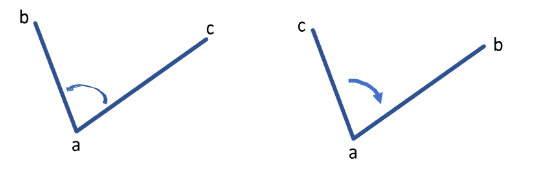
\includegraphics[width=\linewidth]{angel.png}
        \label{angel}
        \caption{شکل سمت چپ زاوره چپ ‌گرد و شکل سمت چپ‌ زاويه راست گرد}
    \end{center}
\end{figure}

پاره‌خط جهت‌دار $\vec{bc}$ (از $b$ به $c$) و نقطه  $a$ که روي راستاي $\vec{bc}$  قرار ندارد داده شده است. زاويه $b\hat{a}c$  در نقطه $a$ منفي يا چپ‌گرد است اگر نقطه $a$ سمت راست  $\vec{bc}$ باشد و مثبت يا راست گرد است اگر نقطه $a$ سمت چپ‌ $\vec{ab}$ باشد.

با توجه به تعريف زاويه چپ‌گرد و راست‌گرد، روش ديگري براي تغيين موقعيت يک نقطه نسبت به يک چندضلعي محدب ارائه مي‌دهيم. 

\subsection{آلگوريتم محاسبه زاويه براي تعيين موقعيت يك نقطه نسبت به چندضلعي}

جهت يادآوري يکبار ديگر صورت مسئله را مرور مي کنيم:
چندضلعي $P$ که مي تواند غير محدب باشد. و نقطه $q$ در صفحه داده شده است. مي خواهيم بررسي کنيم که آيا نقطه $q$ درون چندضلعي است؟

از نقطه $q$ به رئوس چندضلعي وصل کنيم، با کمک نقطه $q$ و اضلاع چندضلعي، مثلث‌هايي ساخته مي‌شود. زواياي رأس $q$ در اين مثلث‌ها را در نظر مي‌گيريم و جمع جبري اين زوايا را محاسبه مي‌کنيم.

براي استفاده از روش زاويه و حل مسئله موقعيت يك نقطه، حول نقطه $q$ به صورت ساعت‌گرد شروع به چرخش مي‌کنيم و با کمک خطوطي که از نقطه $q$  به رئوس چندضلعي وصل شده، به صورت ساعت‌گرد مثلث‌ها را پيمايش مي‌کنيم و زواياي مثلث‌ها در نقطه $q$  را با هم جمع جبري مي‌نماييم؛ اگر جمع جبري زوايا را $W$ بناميم، يکي از دو حالت زير پيش مي‌آيد:

\begin{itemize}
    \item
    اگر مجموع زواياي چرخش برابر 360 درجه باشد نقط $q$ داخل $P$ خواهد بود. ( $W=2\pi$ )
    \item
    اگر مجموع زواياي چرخش برابر صفر باشد نقط $q$ داخل $P$ خواهد بود. ( $W=0$ )
\end{itemize}

\begin{figure}[h!]
    \begin{center}
        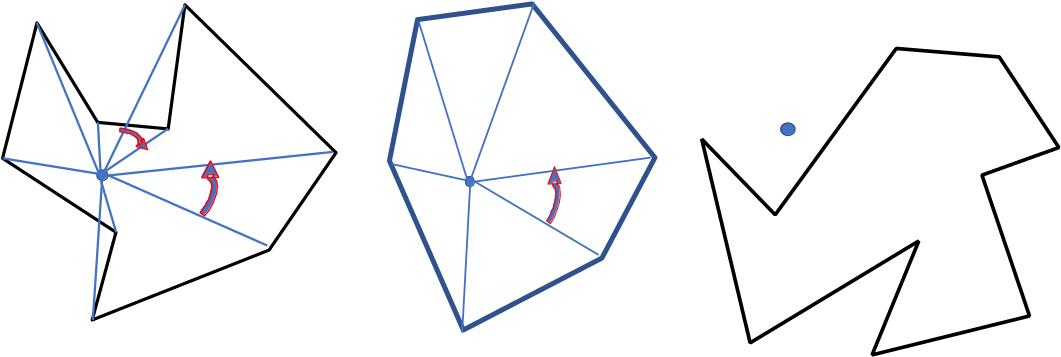
\includegraphics[width=\linewidth]{point_angle.jpg}
        \label{point_angle}
        \caption{ در هر دو شکل سمت چپ، مجموع زواياي چرخش برابر 360 است و نقطه $a$ درون چندضلعي و شکل سمت راست نقطه $q$ خارج چندضلعي مي باشد.}
    \end{center}
\end{figure}

نکته: يک راه ديگر براي بدست آوردن علامت زوايا بهره گيري از ضرب بردارها مي باشد. 

درک نکات فوق چندان دشوار نيست. وقتي مجموع زوايايي که نقطه $q$ با رؤس چندضلعي بطور پي در پي مي سازد برابر 2 است بدين معني است که يک متحرک روي مرز  چندضلعي يک دور کامل به گرد نقطه $q$ چرخيده است. اگر چه ممکن است در بعضي مواقع متحرک بازگشت به عقب داشته باشد که اين در حقيقت همان وقتي است که چندضلعي غير محدب است و زاويه جهت دار نقطه $q$ با رؤس چندضلعي منفي شده است. اگر نقطه $q$ خارج چندضلعي باشد در اين حالت مانند اين است که يک متحرک از نقطه اي روي مرز چندضلعي شروع به حرکت مي کند و بدون اينکه يک دور کامل گرد نقطه $q$ بچرخد به محل اوليه باز مي گردد.

\subsubsection{بررسي موقعيت نقطه در حالات خاص}

با کمک روش زاويه مي‌توان موقعيت هاي خاص نقطه $q$ نسبت به چندضلعي $P$ را نيز بررسي کرد. اين حالت‌ها در شکل زير نشان داده شده اند.

\begin{itemize}
    \item
    اگر $W=\pi$ باشد، آنگاه  نقطه $q$ روي يک ضلع قرار دارد.
    \item
    اگر  $W=\alpha \neq \pi, 2\pi, 0$ آنگاه نقطه $q$ روي يک رأس قرار گرفته است و  $\alpha$ مقدار زاويه داخلي آن رأس را نشان مي‌دهد.
\end{itemize}

\begin{figure}[h!]
    \begin{center}
        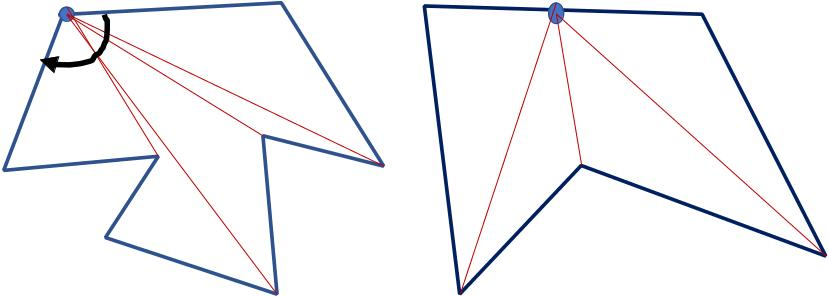
\includegraphics[width=\linewidth]{in_angle.jpg}
        \label{in_angle}
        \caption{شکل سمت چپ $q$ روي يک ضلع قرار داد.. و شکل سمت راست $q$ روي يک رأس قرار گرفته است. و $W$ مقدار زاويه داخلي آن رأس را نشان مي دهد.}
    \end{center}
\end{figure}

\subsection{آناليز الگوريتم}

از آنجا که مي‌توان زاويه چرخش به ازاي هر ضلع از چندضلعي را در زمان ثابت محاسبه کرد و با توجه به اينکه مقدار کليه زواياي داخلي بايد محاسبه گردد، پيچيدگي الگوريتم همانند روش قبلي برابر $O(n)$ خواهد بود.

ممکن است مانند روش ارسال پرتو اين سؤال مطرح شود که دليل اينکه اين آلگوريتم را يک روش افزايشي مي دانيم چيست. پاسخي که در اينجا مي توان داد مشابه آلگوريتم قبلي است. در حقيقت، آلگوريتم اضلاع را يکي يکي مي پيمايد و زاويه اضلاع را نسبت به نقطه داده شده بدست مي آورد. در هر مرحله مقدار زاويه را افزايش و يا کاهش مي دهد تا وقتي که تمام اضلاع چند‌ضلعي را پيمايش کند و به انتها برسد. و تا وقتي که کليه اضلاع بررسي نشده اند هيچ پيش‌بيني صحيح نخواهد بود.

\subsection{تمرين}

امکان پاسخگويي آلگوريتمهاي ارسال پرتو و محاسبه زاويه را در حالتي که چندضلعي داراي سوراخ است، بررسي نماييد.

\section{برش خط}

معمولا دنياي خارج به طور کامل توسط چشم انسان، دوربين و يا سنسور قابل ديد نيست. بلکه به تناسب فراخي دوربين و يا زاويه ديد چشم و يا سنسور، تنها بخشي از دنياي خارج قابل رؤيت مي‌باشد. به عبارت ديگر معمولا تنها برشي از يک تصوير پاناراما را مي‌شود ديد  و اين همان بخشي است که توسط يک ناحيه ديد محصور شده است. براي توضيح بيشتر،  يک چندضلعي را در نظر بگيريد و فرض کنيد يک تصوير توسط اين چندضلعي برش داده شده است. اين چندضلعي مي‌تواند يک ناحيه ديد تصور شود که بخشي از دنياي خارج را برش مي‌زند و تنها همين ناحيه برش‌داده‌شده قابل رؤيت است. بدون شک، اگر ابعاد اين ناحيه ديد بي‌انتها باشد، تمام دنياي خارج ديده مي‌شود؛ ولي اگر ناحيه ديد محدود باشد، بخش‌هايي از دنياي خارج قابل ديدن و بخش‌هايي خارج از ناحيه ديد و غير قابل رؤيت هستند.

مي‌خواهيم بخش‌هايي از اشکال و مناظري را که در يک ناحيه ديد قابل رؤيت هستند، مشخص کنيم. به عبارت ديگر مي‌خواهيم بخش‌هايي از اشکال که درون يک ناحيه ديد قرار مي‌گيرند معين و بخش‌هايي را که خارج ناحيه ديد قرار مي‌گيرند، حذف کنيم.

فرآيند چيدن \footnote{clipping}
(حذف‌كردن) بخشي از يك شکل هندسي كه خارج از يك ناحيه داده‌شده قرار دارد، برش آن شکل ناميده مي‌‌شود.

به تعبيري دقيق‌تر، فرض کنيد مجموعه‌اي از پاره‌خط‌ها و يک ناحيه ديد داده شده است. اين ناحيه ديد به‌ صورت زنجيره بسته‌اي از پاره‌خط‌ها که تشکيل يک چندضلعي را مي‌دهند، قابل بيان است. مي‌خواهيم بخش‌هايي از پاره‌خط‌ها را که درون اين ناحيه قرار مي‌گيرند، مشخص کنيم. به اين کار، برش خط \footnote{‌Line Clipping: The Cyrus-Beck Algorithm}
توسط يک ناحيه گويند.
از آنجا که هر شکلي را با يک چندضلعي مي‌توان تقريب کرد و هر چندضلعي نيز از تعدادي پاره‌خط -که به هم متصل شده‌اند- تشکيل شده است، مي‌توان مسئله را به صورت زير ساده کرد.
مسئله را در ساده‌ترين شکل ممکن بررسي مي‌کنيم؛ حالتي که ناحيه ديد، يک مستطيل است و فضاي بيرون، تنها چند پاره‌خط. اگرچه حالت‌هاي پيچيده‌تر مسئله نسبتا جذاب‌تر و در عين حال سخت‌تر هستند.

\begin{defn}
    مسئله برش خط \footnote{‌Line Clipping Problem}
    : يك ناحيه ديد (مستطيل) و تعدادي پاره‌خط داده شده است. مطلوب است تعيين بخش‌هايي از پاره‌خط‌ها كه درون اين ناحيه ديد قرار دارند.
\end{defn}

\begin{figure}[h!]
    \begin{center}
        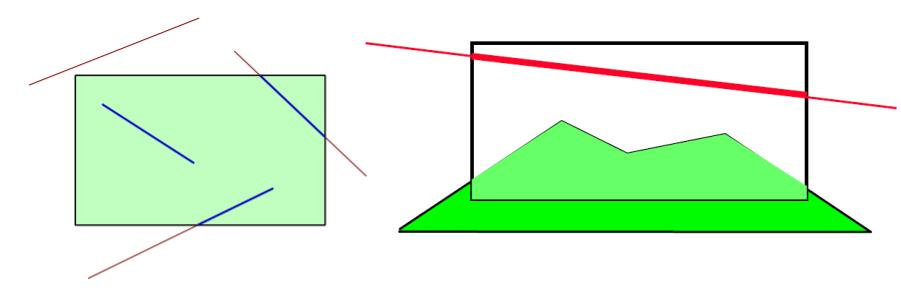
\includegraphics[width=\linewidth]{crop.jpg}
        \label{crop}
        \caption{ناحيه ديد را يک مستطيل در نظر مي‌گيريم و شکل را نيز اجتماعي از تعدادي پاره‌خط که به هم متصل شده‌اند. }
    \end{center}
\end{figure}

چنانچه در گذشته تعريف شد، يک پاره‌خط، ناحيه‌اي از يک خط است که بين دو نقطه محصور شده است. پاره‌خط را مي‌توان به اشکال مختلف نمايش داد. در اينجا پاره‌خط را به صورت پارامتري به شکل زير نمايش مي‌دهيم.

$$ P_t=P_0+(P_1-P_0)t ; 0\leq t\leq 1$$

بنابراين، مجموعه $\{P_0(t),P_1(t),P_2(t),…,P_{n-1}(t)\}$ از پاره‌خط‌ها داده شده است و نيز يک مستطيل که مي‌توان به صورتي کلي، آن را مجموعه‌اي از اضلاع که ناحيه ديد را تشکيل مي‌دهند و بصورت پارامتري به شکل $\{P_L(t),P_R(t),P_T(t),P_B(t)\}$ داده شده‌اند، در نظر گرفت. هدف، عبارت است از تعيين بخش‌هايي از پاره‌خط‌ها که درون اين ناحيه ديد قرار دارند.

اين مسئله را مي توان به چندين روش حل نمود 

\subsection{الگوريتم برش خط}

هر پاره‌خط، با دو نقطه انتهايي‌اش مشخص مي‌شود. يک پاره‌خط و نقاط انتهايي آن را در نظر مي‌گيريم. با توجه به موقعيت پاره‌خط و نقاط انتهايي‌اش، نسبت به مرزهاي ناحيه ديد، حالت‌هاي زير قابل طرح  است.

\begin{itemize}
    \item
    اگر دو سر پاره‌خط درون ناحيه ديد قرار داشته باشد، بدين معني است که  تمام پاره‌خط درون ناحيه ديد قرار دارد و پاره‌خط بطور کامل قابل رؤيت و بنابراين مورد قبول مي‌باشد.
    \item
    اگر دو سر پاره‌خط خارج از يک ضلع ناحيه ديد و سمت راست يک ضلع قرار داشته باشد، تمام پاره‌خط بطور کامل سمت راست آن ضلع قرار دارد و خارج از ناحيه ديد مي‌باشد؛ لذا قابل رؤيت نيست.
    \item
    در صورتي که هيچ کدام از دو حالت بالا اتفاق نيفتد و دو سر پاره‌خط درون ناحيه يا در يک سمت يکي از اضلاع نباشد، در اين صورت نمي‌توان در مورد پاره‌خط صريحا تصميم گرفت. بلکه بايد پاره‌خط در محل برخوردش (يا برخوردهايش) با اضلاع ناحيه ديد، به دو (يا چند) قسمت تقسيم شود و سپس دو مرحله قبل به طور مجزا در مورد هر بخش بررسي گردد. 
\end{itemize}

اکنون مباحث فوق را بيشتر توضيح مي دهيم و سعي مي کنيم يک روش محاسباتي براي مسئله بدست آوريم. 

\begin{figure}[h!]
    \begin{center}
        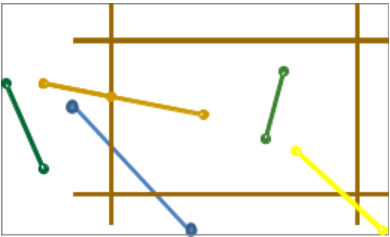
\includegraphics[width=\linewidth]{sq_crop.png}
        \label{sq_crop}
        \caption{وضعيت متفاوت خطوط نسبت به ناحيه ديد}
    \end{center}
\end{figure}


\subsection{محاسبه تقاطع هر خط با اضلاع ناحيه ديد}

ابتدا صفحه را با کمک دو خط موازي عمودي و دو خط موازي افقي حاصل از امتداد اضلاع ناحيه ديد، به 9 زيرناحيه تقسيم مي‌کنيم. سپس يك كد 4 بيتي به هر ناحيه اختصاص مي‌دهيم. آنگاه، با توجه به اينکه رئوس پاره‌خط‌ها در کدام‌ يک از 9 ناحيه قرار دارند، کد ناحيه مربوطه را به آن رأس اختصاص مي‌دهيم. براي اختصاص کد به رئوس پاره‌خط، به شيوه زير عمل مي‌کنيم: \footnote{ اين روش  Cohen-Sutherland Line Clipping نام دارد و روشي ساده و قابل پياده سازي است. لاكن بعضاً نياز به تكرار وجود دارد.روش هاي مؤثر ديگري که مي تواند قابل استفاده باشند عبارتند از: Cyrus-Beck  (parametric lines) و Liang-Barsk }

\begin{figure}[h!]
    \begin{center}
        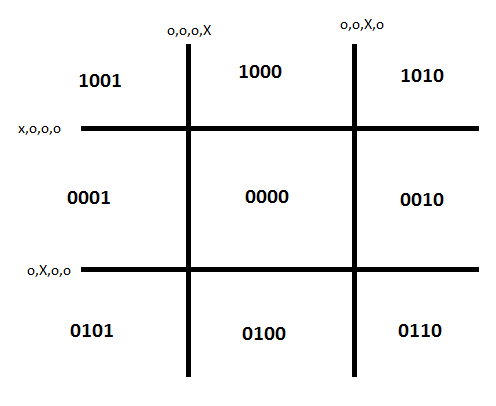
\includegraphics[width=\linewidth]{partition.jpg}
        \label{partition2}
        \caption{ امتداد خطوط بالا ($Y_T$)، پايين ($Y_B$)، راست ($X_R$) و چپ ($X_L$) ، صفحه را به 9 ناحيه تقسيم مي کند }
    \end{center}
\end{figure}

اگر امتداد خطوط ناحيه ديد را خطوط بالا ($Y_T$)، پايين ($Y_B$)، راست ($X_R$)، چپ ($X_L$)، درنظر بگيريم، اين خطوط صفحه را به 9 ناحيه تقسيم مي‌کنند. با مقايسه موقعيت هر رأس نسبت به اين خطوط و موقعيت آن، يک کد 4 بيتي ($Y_T$,$Y_B$,$X_R$,$X_L$)  به آن اختصاص مي‌يابد (شکل بالا را ببينيد).

جهتي را روي اضلاع مستطيل پادساعت‌گرد در نظر مي‌گيريم و با کمک آن، جهتي روي خطوط را مشخص مي‌کنيم. به عبارت ديگر، ابتدا جهت اضلاع مستطيل را پادساعت‌گرد و جهت روي خطوط امتداد اضلاع را همان جهت اضلاع در نظر مي‌گيريم. درنتيجه خطوط ناحيه ديد، جهت پيدا مي کنند. چنانچه يک نقطه سمت راست خط جهت‌دار بود، کد مربوط به آن خط را عدد 1 و چنانچه سمت چپ بود، صفر در نظر مي‌گيريم. 

\begin{figure}[h!]
    \begin{center}
        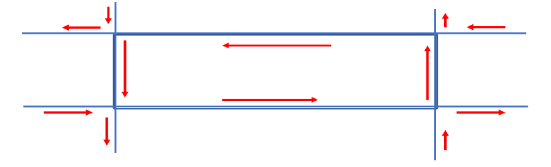
\includegraphics[width=\linewidth]{rec_par.png}
        \label{rec_par}
        \caption{روي اضلاع مستطيل جهت پادساعت‌گرد را در نظر مي‌گيريم و همان جهت را روي خطوط مار بر اضلاع ادامه مي‌دهيم}
    \end{center}
\end{figure}

بنابراين با مقايسه موقعيت يک نقطه نسبت به خطوط ناحيه ديد، به هر نقطه يک كد 4 بيتي اختصاص مي‌يابد. هر بيت بدين صورت مقدار مي‌گيرد که اگر رأس پاره‌خط سمت چپ يک خط باشد، مقدار متناظر آن 1 و اگر سمت راست باشد، صفر خواهد بود. بنابراين هر رأس با چهار خط ناحيه ديد مقايسه مي‌شود و بيت‌ها چهار مقدار صفر و يا 1 مي‌گيرند.

براي تعيين وضعيت پاره‌خط‌ها نسبت به ناحيه ديد، به روش زير عمل مي‌کنيم. 

\begin{itemize}
    \item
    اگر كد هر دو رأس يك خط برابر صفر بود، بدين معني است که رئوس پاره‌خط سمت چپ کليه اضلاع قرار دارند و پاره‌خط درون ناحيه ديد واقع شده است؛ بنابراين تمام پاره‌خط قابل رؤيت است و مورد قبول مي‌باشد و حذف مي شود.
    \item
    در غير اين صورت، كد رئوس پاره‌خط را بيت به بيت با And با هم جمع مي‌كنيم. اگر نتيجه مخالف صفر بود، پاره‌خط به طور کامل سمت راست يکي از اضلاع ناحيه ديد قرار دارد؛ بنابراين پاره‌خط قابل رؤيت نيست و مورد قبول نمي‌باشد و حذف مي شوند
    \item
    در صورتي که نتيجه جمع بيت به بيت دو رأس پاره‌خط با کمک And صفر بود، يک سر پاره‌خط در يک ناحيه از 9 ناحيه و سر ديگر در ناحيه ديگر قرار دارد و بخشي از پاره‌خط ممکن است درون ناحيه ديد باشد. در اين حالت، نه امکان قبول کامل پاره‌خط وجود دارد و نه امکان حذف کامل آن. در اين صورت، بايد تقاطع پاره‌خط را با اضلاع ناحيه ديد بررسي مي‌کنيم و در صورت تقاطع، پاره‌خط را به تعدادي پاره‌خط قابل بررسي تقسيم و روش فوق را در مورد هر بخش به طور جداگانه آزمايش نمود. 
\end{itemize}

\subsection{آناليز آلگوريتم}

کليه مراحل تعيين کدهاي رئوس، بررسي کدهاي دو سر يک پاره‌خط و تصميم‌گيري براي رؤيت‌پذيري پاره‌خط‌ها، در زمان O1 انجام مي‌شوند؛ بنابراين براي يک دسته On پاره‌خط، زمان آلگوريتم عبارت خواهد بود از: 

$$T(n)=O(n)\times O(1)=O(n)$$

روش جمع منطقي And بصورت زير است.

$$1 \rightarrow 1+1$$
$$0 \rightarrow 0+0$$
$$0 \rightarrow 1+0$$
$$0 \rightarrow 0+1$$

\section{برش چند ضلعي}

اگر قرار باشد در مورد برش يک شکل مستقيما تصميم بگيريم، کار مقداري سخت‌تر خواهد شد. بدون شک برش چند ضلعي \footnote{ Polygon Clipping problem: Sutherland-Hodgman Algorithm}
از برش خطوط مشکل تر است. در کلي‌ترين شکل مي‌توان مسئله برش يک چندضلعي \footnote{SubjectPoly}
را به شکل زير مطرح نمود.

\begin{figure}[h!]
    \begin{center}
        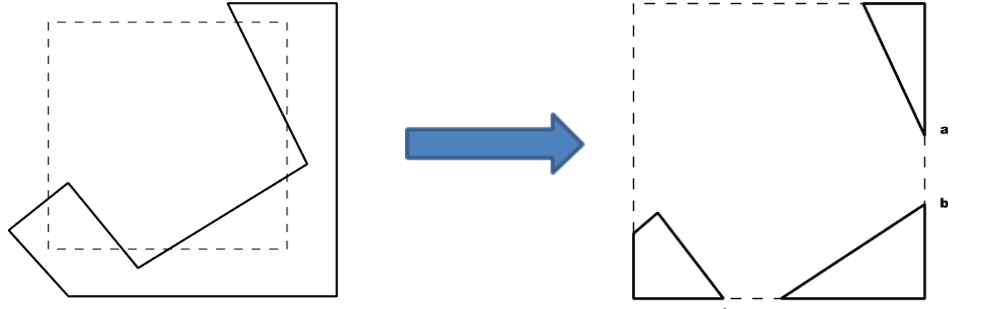
\includegraphics[width=\linewidth]{pol_clip.png}
        \label{pol_clip}
        \caption{چندضلعي دلخواه $S$ و چندضلعي محدب $P$ داده شده است. هدف برش $S$ توسط $P$ مي‌باشد.}
    \end{center}
\end{figure}

ورودي مسئله: يک محدوده ديد که مي تواند يک مستطيل باشد و يا در حالت کلي يک چند ضلعي 

خروجي مسئله: يک يا تعدادي چندضلعي و يا هيچ.

حل اين مسئله با روش سايرس-يک صورت مي گيرد. توضيح آن طولاني و نسبتاً خسته کننده است. اما در يک نگاه کلي و بصورتي خلاصه اين روش به شکل زير عمل مي کند.

ايده اصلي الگوريتم به صورت زير است:

\begin{itemize}
    \item
    هر ضلع از ناحيه ديد را بصورت جداگانه در نظر مي‌گيريم.
    \item
    چندضلعي را به وسيله ضلع مذکور با روش سايرس- بک \footnote{ Line Clipping: Cyrus-Beck Algorithm} برش مي‌زنيم.
    \item
    برش چندضلعي را توسط کليه اضلاع ناحيه ديد يکي يکي انجام مي دهيم.
    \item
    با اتمام کليه اضلاع، برش شکل به پايان مي‌رسد.
\end{itemize}

\begin{figure}[h!]
    \begin{center}
        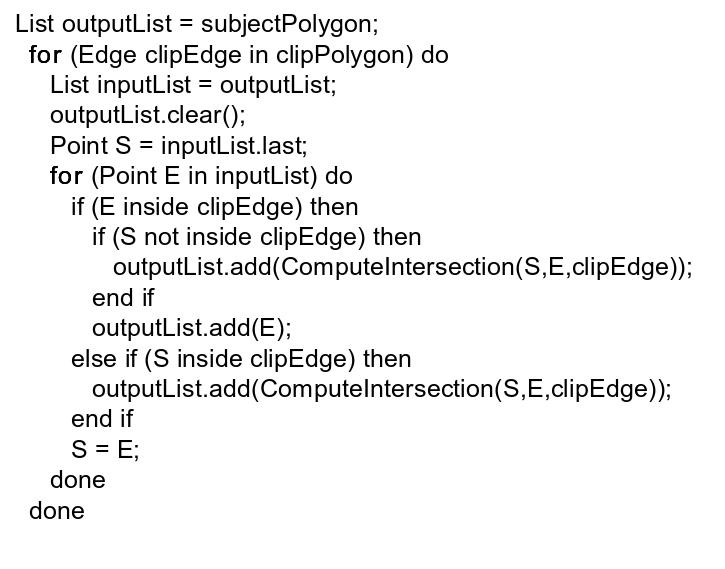
\includegraphics[width=\linewidth]{clip_algo.jpg}
        \label{clip_algo}
        \caption{شبه کد الگوريتم به صورت بالا است}
    \end{center}
\end{figure}
    

روش سايرس- بک که از آن در بالا نام برده شد به صورتي بسيار کلي به روش زير عمل مي کند.

\begin{figure}[h!]
    \begin{center}
        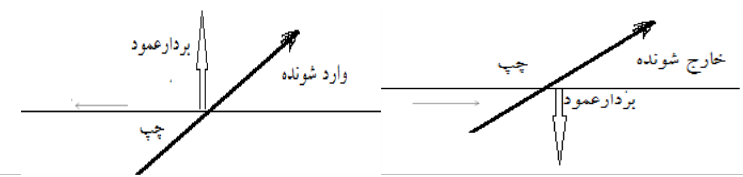
\includegraphics[width=\linewidth]{cyres.png}
        \label{cyres}
        \caption{يک ضلع واردشونده بالقوه (خارج‌شونده بالقوه) است؛ اگر زوايه بين N  (بردار عمود بر مرز ناحيه ديد) و s (ضلع مذکور) يک زاويه ساعت‌گرد(پادساعت‌گرد) باشد.}
    \end{center}
\end{figure}

فرض کنيد مستطيل $P$ که همان ناحيه ديد است و پاره‌خط $S$ که يک يال از شکل مورد نظر است، داده شده‌اند. مي خواهيم پاره‌خط $S$ را توسط مستطيل $P$ برش بزنيم. به عبارت ديگر هدف يافتن قسمتي از $S$ است كه در داخل$P$ قرار دارد. جهتي را براي چندضلعي $P$ و جهتي را نيز براي پاره خط $S$ در نظر مي‌گيريم. با توجه به موقعيت $S$ نسبت به $P$ دو نوع موقعيت متفاوت براي $S$ تعريف مي‌کنيم.

\begin{itemize}
    \item
    وارد‌شونده بالقوه \footnote{potentially entering-pe}
    \item
    خارج‌شونده بالقوه \footnote{potentially leaving-pl}
\end{itemize}

با بررسي دو نوع برخورد متفاوت وارد‌شونده بالقوه و خارج‌شونده بالقوه و ترتيب قرارگرفتن پي در پي آنها روي يال $S$ مي‌توان در مورد وضعيت خط$S$  نسبت به مستطيل ناحيه ديد نظر داد. (شکل 5 را ببينيد) 

با توجه به موقعيت‌هاي  واردشونده و يا خارج‌شونده و نحوه تکرار اين‌ها، پاره‌خط $S$ نسبت به $P$ يکي از چهار شکل شکل \ref{in_out} را خواهد داشت

\begin{figure}[h!]
    \begin{center}
        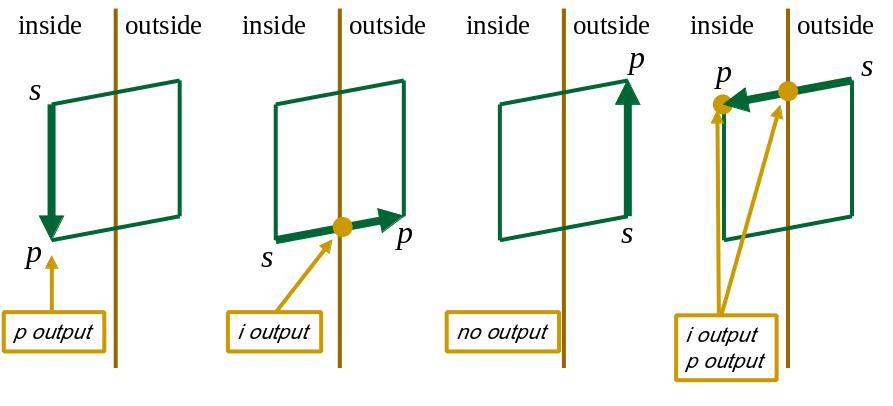
\includegraphics[width=\linewidth]{in_out.jpg}
        \label{in_out}
        \caption{ با توجه به موقعيت يک يال نسبت به ضلع ناحيه ديد خروجي هاي برنامه مي تواند متفاوت باشد.}
    \end{center}
\end{figure}

ممکن است اين توضيح ابهامات بيشتري در ذهن شما ايجاد کرده باشد و سؤالات متعددي برايتان مطرح شده باشد ولي متاسفانه توضيح بيشتر به مقدمات نسبتا زيادي نياز دارد که خارج از عهده اين کتاب است.

\begin{figure}[h!]
    \begin{center}
        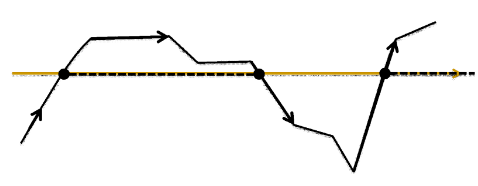
\includegraphics[width=\linewidth]{p_clip.png}
        \label{p_clip}
        \caption{ برش هر چندضلعي را با بررسي جداگانه وضعيت يال‌هايش نسبت به ناحيه ديد مي‌توان  مشخص کرد}
    \end{center}
\end{figure}

\section{توليد چندضلعي‌هاي ساده تصادفي در فضاي دو بعدي}

\subsection{مقدمه و کاربردها}
توليد چندضلعي ساده تصادفي با کمک مجموعه‌اي از نقاط، از جمله مسائل مطرح در هندسه محاسباتي مي‌باشد. اين مسئله در زمينه‌هاي مختلف گرافيک کامپيوتري، نظير خلق تصاوير پديده‌هاي طبيعي تصادفي (مانند پديده ابر و سطح زمين)، به طور گسترده‌اي مورد استفاده قرار مي‌گيرد. 

اگر به خاطر داشته باشيد قبلا در بخش مربوط به ساخت چندضلعي ستاره شکل توضيح داديم که با مجموعه اي از نقاط مي توان يک چندضلعي ستاره شکل ساخت. روشهاي ساده ديگري نيز براي ساخت يک چندضلعي با کمک مجموعه‌اي از نقاط وجود دارد. لاکن هيچکدام از اين روشها در ساخت چندضلعي نقاط را بطور تصادفي بکار نمي گيرند و يک چندضلعي تصادفي به عنوان خروجي آلگوريتم بدست نمي دهند.

واقعيت اين است که هيچ روش خاصي با پيچيدگي زماني چندجمله‌اي براي توليد چندضلعي ساده تصادفي با توزيع يکنواخت وجود ندارد. لاکن در اين بخش، دو روش‌ افزايشي براي حل اين مسئله توضيح داده مي‌شود. اين روش‌ها قادر به پوشش تمام فضاي مسئله نيستند؛ به عبارت ديگر، چندضلعي توليدشده تمام نقاط ورودي مسئله را مورد استفاده قرار نمي‌دهد و نيز چندضلعي‌هاي ممکن را با توزيع يکنواخت توليد نمي‌کند؛ ولي پيچيدگي زماني چندجمله‌اي دارد.  

توليد چندضلعي‌ ساده تصادفي در زمينه‌هاي زير کاربرد دارد:

\begin{itemize}
    \item
    توليد چندضلعي‌ ساده تصادفي براي تست درستي و يا براي بررسي ميزان مصرف پردازنده توسط الگوريتم‌هايي که روي چندضلعي‌ها اعمال مي‌شوند و ورودي آن‌ها چندضلعي است.
    \item
    توليد چندضلعي‌ ساده تصادفي براي ارائه انواع وسيعي از شکل‌هاي گرافيک رايانه‌اي، بينايي ماشين، تشخيص الگو و نيز براي الگوي يک مانع براي يک ربات و ديگر زمينههاي هندسي استفاده مي‌شود.
\end{itemize}

در مورد کاربرد اول، لازم به توضيح است که براي آزمودن درستي يک الگوريتم، معمولاً تلاش مي‌کنيم که ايرادهاي \footnote{bug} الگوريتم را مشخص کنيم. براي اين ‌کار، معمولاً داده‌هايي را که به صورت تصادفي توليد شده‌اند به عنوان ورودي به الگوريتم مي‌دهيم و نتيجه را بررسي مي‌کنيم.
کاربرد دوم، توليد چندضلعي‌هاي تصادفي براي آزمودن ميزان مصرف پردازنده براي يک الگوريتم است. معمولاً براي آزمودن ميزان مصرف پردازنده، نياز به داده‌هاي زيادي داريم که در عمل، توليد و به دست آوردن اين مقدار داده غيرممکن است. بنابراين براي آزمودن مصرف پردازنده از داده‌هايي که به صورت تصادفي توليد شده‌اند استفاده مي‌کنيم.

\subsection{الگوريتم افزايشي: روش اول}

با استفاده از الگوريتم اوير\footnote{در سال 1996 توماس اوير (Thomas Auer )يک الگوريتم افزايشي ارائه کرد که مرحله به مرحله اقدام به توليد چندضلعي مي‌کند و در هر مرحله، يک راس را به چندضلعي اضافه مي‌نمايد. پيچيدگي زماني مسئله O(n2) و پيچيدگي فضايي آن O(n) است [2]. متاسفانه الگوريتم افزايشي اوير قادر به توليد تمام چندضلعي‌ها نيست؛ بلکه با توزيعي غيريکنواخت چندضلعي‌ها را توليد مي‌کند.}
، به روش افزايشي و مرحله به مرحله اقدام به ساخت چندضلعي مي‌کنيم.  در يک توضيح کلي، به اين شکل عمل مي‌کنيم که ابتدا از يک نقطه و سپس از دو نقطه شروع مي‌کنيم و در مرحله k ام، نقطه جديد sk را به چندضلعي Pk-1 که در مرحله k-1 توليد شده اضافه مي نماييم. اضافه‌شدن يک رأس جديد به چندضلعي به اين شکل است که يکي از يال‌هايي را که از sk به‌ طور کامل قابل رويت است، مانند (vi,vi+1) از چندضلعي Pk-1  حذف و يال‌هاي (vi,sk) و (sk,vi+1) را به Pk-1 اضافه مي‌نماييم. اضافه‌کردن sk به Pk-1 بايد به شکلي انجام شود که تضمين کند n-k نقطه باقيمانده نيز مي‌توانند به چندضلعي اضافه شوند. در اين مورد بايد مراقب بود و نقاط را به شکل مناسبي انتخاب کرد؛ زيرا همان‌طور که در شکل 8 و شکل 9 مشخص است، ممکن است نقطه‌اي در داخل يا خارج از چندضلعي وجود داشته باشد که هيچ‌يک از يال‌ها را به‌صورت کامل نبيند. \footnote{ORourke, J., and M.Virmani. 1991. Generating random polygons. Technical Report 11. Cs Dept. Smith College, Northampton, MA. 38-44.}

\begin{figure}[h!]
    \begin{center}
        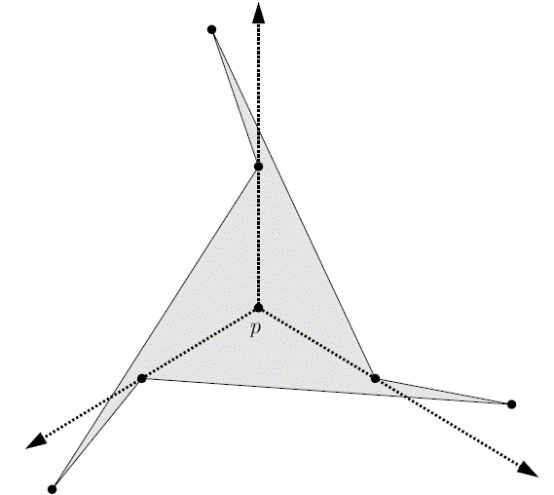
\includegraphics[width=\linewidth]{see_exception.jpg}
        \label{see_exception}
        \caption{نقطه p  درون چندضلعي نمي تواند هيچ‌ يک از يال‌هاي چندضلعي را ببيند.}
    \end{center}
\end{figure}

\begin{figure}[h!]
    \begin{center}
        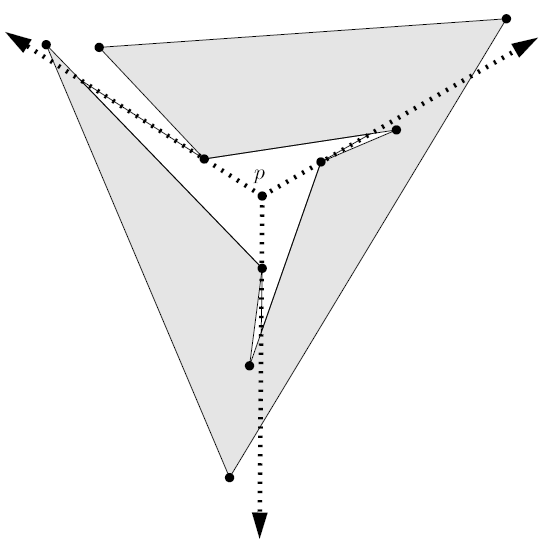
\includegraphics[width=\linewidth]{see_exception2.jpg}
        \label{see_exception2}
        \caption{ نقطه $p$  خارج چندضلعي نمي تواند هيچ‌ يک از يال‌هاي چندضلعي را ببيند.}
    \end{center}
\end{figure}

براي رفع اين مشکل کافي است نقطه‌ي جديد $p$ را از خارج پوش محدب ( $CH(Q)$ ) انتخاب کنيم، در اين صورت مي‌توان ثابت کرد که حداقل $p$ يک يال $Q$ را به ‌طور کامل قابل مي‌بيند. بنابراين، اگر مجموعه $S_k$ را به صورت زير تعريف کنيم:     $S_k\leftarrow S\{s_1,…, s_{k-1}\}$

$S_k$ شامل تمام نقاط مجموعه $S$ به جز نقاط $P_{k-1}=\{s1,…, s_{k-1}\}$ مي‌باشد. در مرحله$k+1$  ام $s_k$ را انتخاب کرده و با کمک آن $P_k$  را مي‌سازيم. اگر تضمين شود که هيچ نقطه‌اي از $S_{k+1}$ يعني نقاط باقيمانده در مرحله$k+1$ بعد از مرحله درون $CH(P_k)$ قرار نمي‌گيرد، مي‌توان اثبات کرد که تمام مرحله‌هاي توليد چندضلعي قابل انجام است.


\begin{latin}
\begin{verbatim}
    Algorithm SteadyGrowth(S):

    Select s1ϵ S at random.     O(1) 
    Select s2 ϵ S\{s1} at random.      O(1) 
    Let s3 := S\{s1,s2}.     O(1) 
    Let P3 :=CHs1,s2,s3.    O(1) 
    for  k=4  to  n  do     O(n) 
    Pick a point sk such that all points  s  Sk+1  lie outside of CHPk-1sk   O(n)
            Insert sk into the convex hull. 
            Find all edges that are visible from sk.     O(n) 
            Pick one visible edge e = vi,vi+1at random.     O1
            Pk is obtained from Pk-1 by replacing the edge e with the 
            edges  vi,skand sk,vi+1 .      O(1)
            Let Sk+1 := Sk\{sk}.     O(1)  
\end{verbatim}
\end{latin}

قابل ذکر است که الگوريتم روي يک مجموعه نقاط مرحله به مرحله شرح داده شده است. براي هر مرحله از الگوريتم، از يک شکل کمک گرفته شده است و نقطه‌ انتخاب شده و چندضلعي توليد شده در آن مرحله نشان داده شده است. 

\begin{figure}[h!]
    \begin{center}
        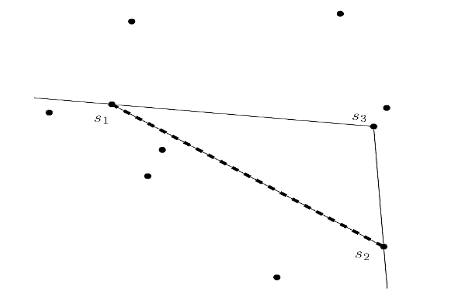
\includegraphics[width=\linewidth]{simp1.png}
        \label{simp1}
        \caption{در مرحله اول دو نقطه $s_1$ و $s_2$ به‌صورت تصادفي انتخاب مي شوند.}
    \end{center}
\end{figure}


در شکل \ref{simp1} مرحله اول الگوريتم نشان داده شده است که دو نقطه $s_1$ و $s_2$ به‌صورت تصادفي انتخاب شده‌اند.
$s3 \leftarrow S\\\{s1,s2\}$   طوري انتخاب مي‌شود که درون $CH(p_2 \cup \{s_3\})$ هيچ نقطه‌اي قرار نداشته باشد. $s_3$ به $s_1$ و $s_2$ وصل مي‌شود. 

\begin{figure}[h!]
    \begin{center}
        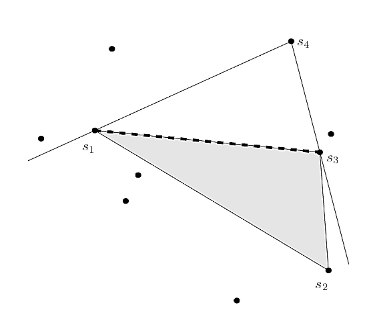
\includegraphics[width=\linewidth]{simp2.png}
        \label{simp2}
        \caption{s4 براي اضافه‌شدن به $P_3$ انتخاب‌ شده است در اين حالت هيچ نقطه‌اي درون $CH(p_3 \cup \{s_4\})$ وجود ندارد.}
    \end{center}
\end{figure}

شکل \ref{simp2} مرحله دوم الگوريتم را نمايش مي‌دهد. راس $s_4$ براي اضافه‌شدن به $P_3$ انتخاب‌ شده است و هيچ نقطه‌اي درون $CH(p_3 \cup \{s_4\})$ وجود ندارد. بنابراين نقطه $s_4$ مشکلي براي ادامه کار آلگوريتم بوجود نمي آورد. يال $s_3$ تا $s_1$ توسط نقطه $s_4$ قابل رويت است بنابراين يال $(s_1,s_3)$ حذف مي‌شود و يال‌هاي $(s_4,s_3)$ و $(s_1,s_4)$ به چندضلعي اضافه مي‌شوند.

\begin{figure}[h!]
    \begin{center}
        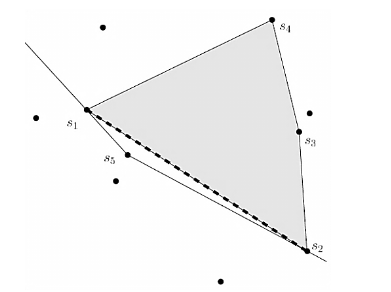
\includegraphics[width=\linewidth]{simp3.png}
        \label{simp3}
        \caption{نقطه $s_5$ به چندضلعي اضافه‌ و يال $(s_1,s_2)$ که به طور کامل ديده مي شود حذف و يال‌هاي $(s_1,s_3)$ و $(s_2,s_3)$ اضافه مي‌شوند.}
    \end{center}
\end{figure}

شکل \ref{simp3} مرحله سوم الگوريتم را نمايش مي‌دهد که نقطه $s_5$ براي اضافه‌شدن به چندضلعي انتخاب شده است. اين نقطه تنها يال $(s_1,s_2)$ از $P_4$ را به‌ طور کامل مي‌بيند، پس يال $(s_1,s_2)$ حذف و يال‌هاي $(s_1,s_3)$ و $(s_2,s_3)$ به چندضلعي اضافه مي‌شوند.

\begin{figure}[h!]
    \begin{center}
        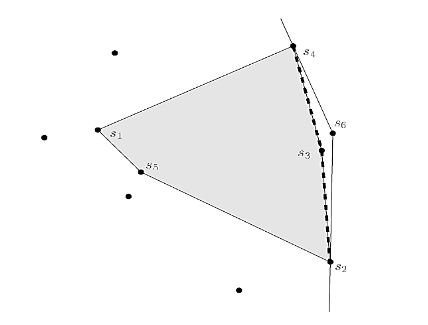
\includegraphics[width=\linewidth]{simp4.png}
        \label{simp4}
        \caption{از بين دو يالي که نقطه جديد $s_6$  مي بيند، $(s_4,s_3)$ به تصادف حذف و يال‌هاي $(s_6,s_3)$ و $(s_6,s_4)$ اضافه مي‌شوند.}
    \end{center}
\end{figure}

در مرحله چهارم که در شکل \ref{simp4} نشان داده شده است، نقطه $s_6$ به چندضلعي اضافه مي‌شود. $s_6$ دو يال $(s_4,s_3)$ و $(s_2,s_3)$، از $P_5$ را به ‌طور کامل مي‌بيند. پس از بين اين دو، يال $(s_4,s_3)$ را به تصادف انتخاب و از چندضلعي حذف و يال‌هاي $(s_6,s_3)$ و $(s_6,s_4)$ به چندضلعي اضافه مي‌شوند.

\begin{figure}[h!]
    \begin{center}
        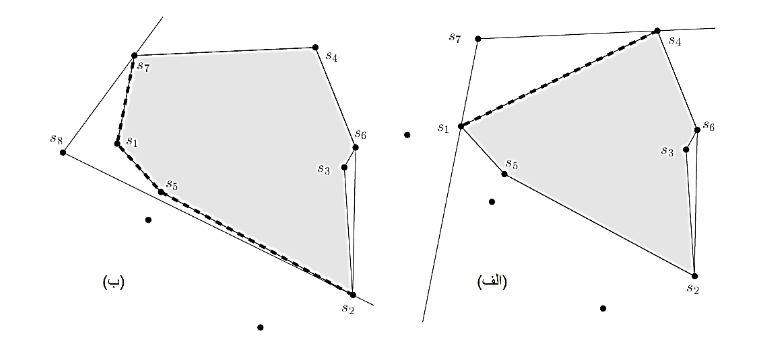
\includegraphics[width=\linewidth]{simp5.png}
        \label{simp5}
        \caption{(الف) مرحله پنجم و (ب) مرحله ششم الگوريتم رشد پي‌درپي}
    \end{center}
\end{figure}

\begin{figure}[h!]
    \begin{center}
        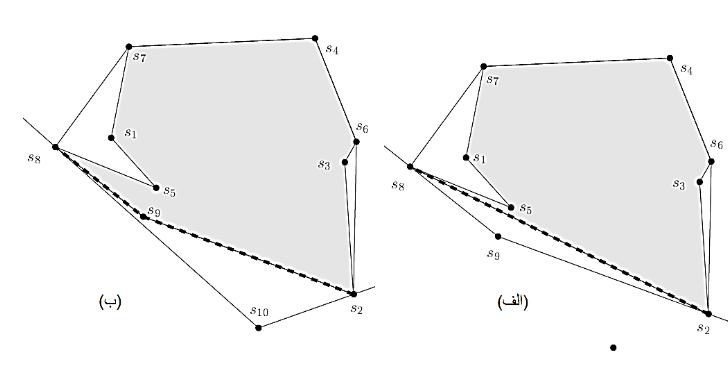
\includegraphics[width=\linewidth]{simp6.png}
        \label{simp6}
        \caption{(الف) مرحله هفتم و (ب) مرحله هشتم الگوريتم رشد پي‌درپي}
    \end{center}
\end{figure}

\begin{figure}[h!]
    \begin{center}
        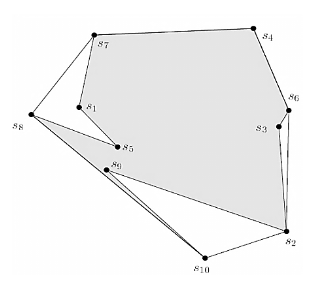
\includegraphics[width=\linewidth]{simp7.png}
        \label{simp7}
        \caption{مرحله پاياني الگوريتم رشد پي‌درپي}
    \end{center}
\end{figure}

در مرحله‌هاي 5، 6، 7، 8 و 9 نيز عملياتي مشابه مرحله‌هاي قبلي انجام مي‌شود. شکل‌هاي‌ 14 ،15 و 16 اين مرحله‌ها را در کنار هم نشان داده اند. شکل‌ \ref{simp5} مرحله 5 و 6 الگوريتم رشد پي‌درپي را نشان مي‌دهد، که در مرحله پنجم (شکل الف) چندضلعي با هفت رأس و در مرحله ششم (شکل ب) چندضلعي با هشت ضلع توليد مي‌شود. شکل \ref{simp5} مرحله 7 و 8 الگوريتم رشد پي‌درپي را نشان مي‌دهد که در مرحله هفتم (شکل الف) چندضلعي با نه رأس و در مرحله هشتم (شکل ب) چندضلعي با ده ضلع توليد شده است. شکل \ref{simp6} مرحله پاياني الگوريتم را نشان مي‌دهد.

مي توان ثابت نمو پيچيدگي زماني مسئله $O(n^2)$ و پيچيدگي فضايي آن $O(n)$ است. \footnote{Auer, T., and Martin Held. 1996. Rpg-Heuristics for the generation of random polygons. In Proc. 8th Canadian Conference on Computational Geometry. 38-44.}

\section{الگوريتم افزايشي توليد چندضلعي ساده - روش دوم}

\begin{figure}[h!]
    \begin{center}
        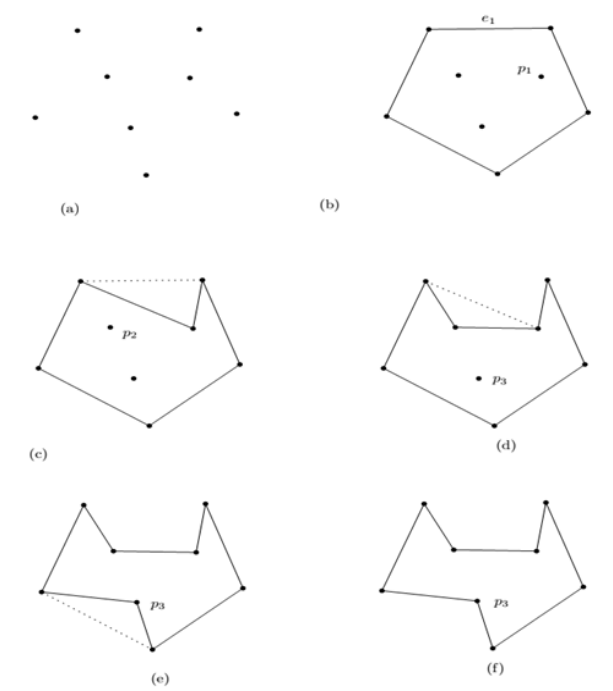
\includegraphics[width=\linewidth]{simp_sec.png}
        \label{simp_sec}
        \caption{(b): ابتدا پوش محدب نقاط داده‌شده را محاسبه مي کنيم (c): يک نقطه را انتخاب و دو سر يکي از يال‌هايي که توسط نقطه قابل رؤيت هستند را  به نقطه متصل و خود  يال را حذف مي‌کنيم.  (d-f): اين عمل را براي کليه نقاط باقي مانده تکرار مي کنيم.}
    \end{center}
\end{figure}

در اين روش که مقداري با آلگوريتم قبلي متفاوت است، از روش افزايشي براي توليد چندضلعي ساده با کمک مجموعه‌اي از نقاط داده شده استفاده مي‌کنيم. ابتدا يک پوش محدب از مجموعه نقاط داده‌شده را محاسبه مي‌کنيم. سپس با کمک پوش محدب مرحله به مرحله به چندضلعي مورد نظر مي‌رسيم. به عنوان توضيح بيشتر، در اين آلگوريتم ابتدا توسط يک آلگوريتم دلخواه (براي مثال آلگوريتم گراهام)  پوش محدب مجموعه نقاط داده شده را محاسبه مي‌کنيم. اگر هيچ نقطه‌اي درون پوش باقي نماند که مسئله حل شده است و پوش محدب جواب مسئله خواهد بود. در غير اينصورت همه نقاط باقي‌مانده درون پوش محدب قرار مي‌گيرند و بايد تا حد ممکن به چندضلعي اضافه شوند. بصورت تصادفي يکي از نقاط را انتخاب و $v_i$  مي ناميم. سپس يال‌هايي را که از $v_i$ قابل رؤيت هستند محاسبه و از بين آنها يکي را به صورت تصادفي انتخاب مي‌کنيم. دو سر آن يال را به نقطه $v_i$ متصل و خود  يال موردنظر را حذف مي‌کنيم. با اين کار يک قدم به جواب نزديکتر شده‌ايم. بعد از آن نقاط را يکي يکي انتخاب و عملي را که در مورد $v_i$  انجام داده‌ايم تکرار مي‌کنيم. اين کار را تکرار مي کنيم تا جايي که ديگر نقطه اي نماند که بتواند با اين روش به چندضلعي اضافه شود. در پايان ما يک چندضلعي ساده داريم که با کمک نقاط داده شده که به طور تصادفي يکي يکي انتخاب شده اند ساخته شده است. شکل \ref{simp_sec} را ملاحظه کنيد.

\begin{figure}[h!]
    \begin{center}
        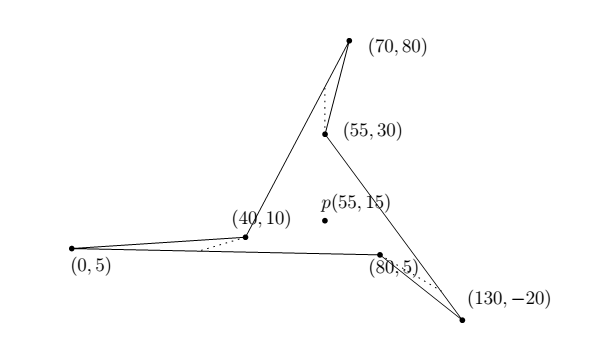
\includegraphics[width=\linewidth]{simp_sec2.jpg}
        \label{simp_sec2}
        \caption{حالت خاصي که با کمک الگوريتم افزايشي 2 به پايان نمي رسد.}
    \end{center}
\end{figure}

\begin{figure}[h!]
    \begin{center}
        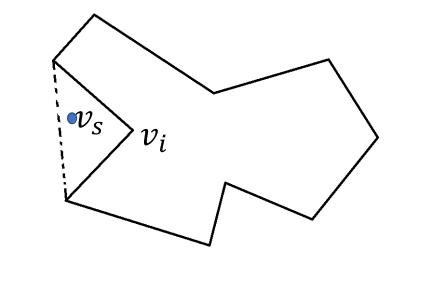
\includegraphics[width=\linewidth]{simp_sec3.jpg}
        \label{simp_sec3}
        \caption{مثلث ساخت شده توسط نقطه‌ي $v_i$  و ضلع قابل رؤيت چندضلعي شامل نقطه ملاقات نشده $v_s$ است.}
    \end{center}
\end{figure}

مسائل زيبايي در زمينه ساخت دياگرام ورونوي و مثلث بندي دلوني وجود دارد که براي حل آنها از روش افزايشي استفاده مي کنيم. بررسي اين مسائل را به آينده موکول مي‌کنيم. چرا که طرح آنها نياز به مقدمات نسبتا زيادي دارد که پرداختن به آنها در اينجا امکان پذير نيست.

\subsection{تمرين}

مسئله1: چندضلعي $Q$ و نقطه‌ي $p$ در خارج پوش محدب ( $CH(Q)$ ) داده شده است. ثابت کنيد $p$ حداقل يک يال $Q$ را به‌ طور کامل مي‌تواند ببيند. آلگوريتمي براي يافتن ضلعي از چندضلعي $Q$ که توسط نقطه‌ي $p$ قابل رؤيت است، ارائه دهيد.
مسئله2: در آلگوريتم بالا تعريف مي‌کنيم:  $S_k\leftarrow S\{s_1,…, s_{k-1}\}$ و در مرحلهk+1  ام براي ساختن Pk نقطه sk را به گونه‌اي انتخاب مي‌کنيم که هيچ نقطه‌اي از $S_k\{s_k\}$ درون $CH(P_k)$ قرار ‌نگيرد.  آلگوريتمي براي انتخاب $sk$  ارائه نماييد. 

مسئله 3: در روش الگوريتم افزايشي رشد پي‌در‌پي  چندضلعي به‌وجودآمده در مرحله $k$ ام را با $P_{k-1}$  نشان مي‌دهيم.

 الگوريتمي ارائه دهيد که مرحله $k+1$  ام را انجام دهد. به عبارت ديگر، آلگوريتمي که روش انتخاب و افزودن نقطه  $s_kبه$ $P_{k-1}$ و ساختن  $P_k$ را توضيح دهد.

\subsection{مسائل}

\colorbox{yellow}{بخش GA96-3-6 اضافه نشده است. و بايستي در بخش مثلث بندي دلوني بيايد.}

\chapter{الگوريتم‌هاي جاروي صفحه}

\section{مقدمه  و کاربرد}

آلگوريتم جاروي صفحه \footnote{Plane–Sweep Algorithm} ، يک روش ساده و در عين حال موثر براي حل مسائل هندسي است. اين روش عمدتا براي حل مسائلي از هندسه مفيد است که به نحوي به بررسي خاصيتي در مورد اشياي هندسي در صفحه مي‌پردازند. الگوريتم‌هاي جاروي صفحه را مي‌توان نوع خاصي از الگوريتم‌هاي افزايشي دانست؛ زيرا با يک روش پيمايش، داده‌ها را يکي يکي بررسي و در هر مرحله، جواب مرحله قبلي را بهبود مي‌بخشد و تا وقتي کليه داده‌ها بررسي نشده‌اند، پاسخ نهايي مسئله مشخص نمي‌باشد.

روش خط جارو احتمالا از آلگوريتم خط اسکن که در تحليل گرافيک کامپيوتري کاربرد دارد و يا از آلگوريتم هاي طراحي مدارهاي يکپارچه \footnote{Integrated circuite layout design} که در آن توصيف هندسي يک مدار IC به دليل گستردگي در حافظه امکان پذير نمي باشد الهام گرفته است.  

بدين منظور که يک ديد کلي نسبت به نحوه عملکرد اين آلگوريتم داشته باشيم به دو مثال زير توجه کنيد.

فرض کنيد از شما خواسته شده است در يک اطاق بزرگ که با موکت فرش شده است شيئ بسيار کوچکي را بيابيد. با اين فرض که هيچ ايده  اوليه‌اي براي محل شيئ نداريد. براي يافتن آن از چه روشي استفاده مي کنيد؟ بدون شک باید از روشي استفاده کنید که به شما کمک کند با اطمينان در انتهاي جستجو شيئ را بيابيد و نيز زمان جستجو به حداقل برسد در حاليکه هيج نقطه اي را دو بار جستجو نکرده ايد. آيا ترجيح مي دهيد بدون يک طراحي حرکت و بطور تصادفي به هر گوشه و ناحيه اطاق سرک بکشيد و آنجا را جستجو کنيد، يا با نظمي مشخص از گوشه اي و سمتي آغاز و بطور پيوسته ناحيه جستجو شده را گسترش دهيد. اجازه دهيد بجاي توضيح بيشتر مثال ديگري را با هم دنبال کنيم.

\end{document}
